\documentclass[rgb,dvipsnames]{beamer}
\usepackage[english]{babel}
\usepackage{geometry}
\usepackage[utf8]{inputenc}
\usepackage{colortbl}
\usepackage{listings}
\usepackage{adjustbox}
\usepackage{amsmath}
\usepackage{multirow}
\usepackage{tabularx}
\usepackage{tikz}
\usepackage[linewidth=1pt]{mdframed}

% Graphics
\usepackage{graphicx}

% Font
\usepackage{paratype}
\setbeamerfont{frametitle}{family=\bf}

% Beamer theme settings
\usecolortheme{seagull}
\usenavigationsymbolstemplate{} % no navigation buttons

\newcommand{\Fn}{\ensuremath{\lambda}}

\lstdefinelanguage{Futhark}
{keywords={fun,if,then,else,loop,do,map,reduce,filter,scan,redomap,transpose,rearrange,reshape,iota,replicate,let,in,for,while,with,f32,i32,i8,u8,zip,stream_red,unsafe,local},%
  sensitive=true,%
  comment=[l]{--},%
  string=[b]",%
  literate={\\}{\Fn}{1} {->}{$\rightarrow$}{1} {<-}{$\leftarrow$}{1},
  moredelim=**[is][\color{red}]{@}{@},
  moredelim=**[is][\color{blue}]{!}{!},
}

\lstdefinelanguage{none}{
  identifierstyle=
}

\lstset{
  language=Futhark,
  basicstyle=\footnotesize
}

\title{Design and Implementation of the Futhark Programming Language}
\date{15th of November 2017}
\author{Troels Henriksen}
\institute{DIKU\\
  University of Copenhagen}

\begin{document}

\usebackgroundtemplate{
\tikz[overlay,remember picture] \node[opacity=0.4, at=(current page.center)] {
   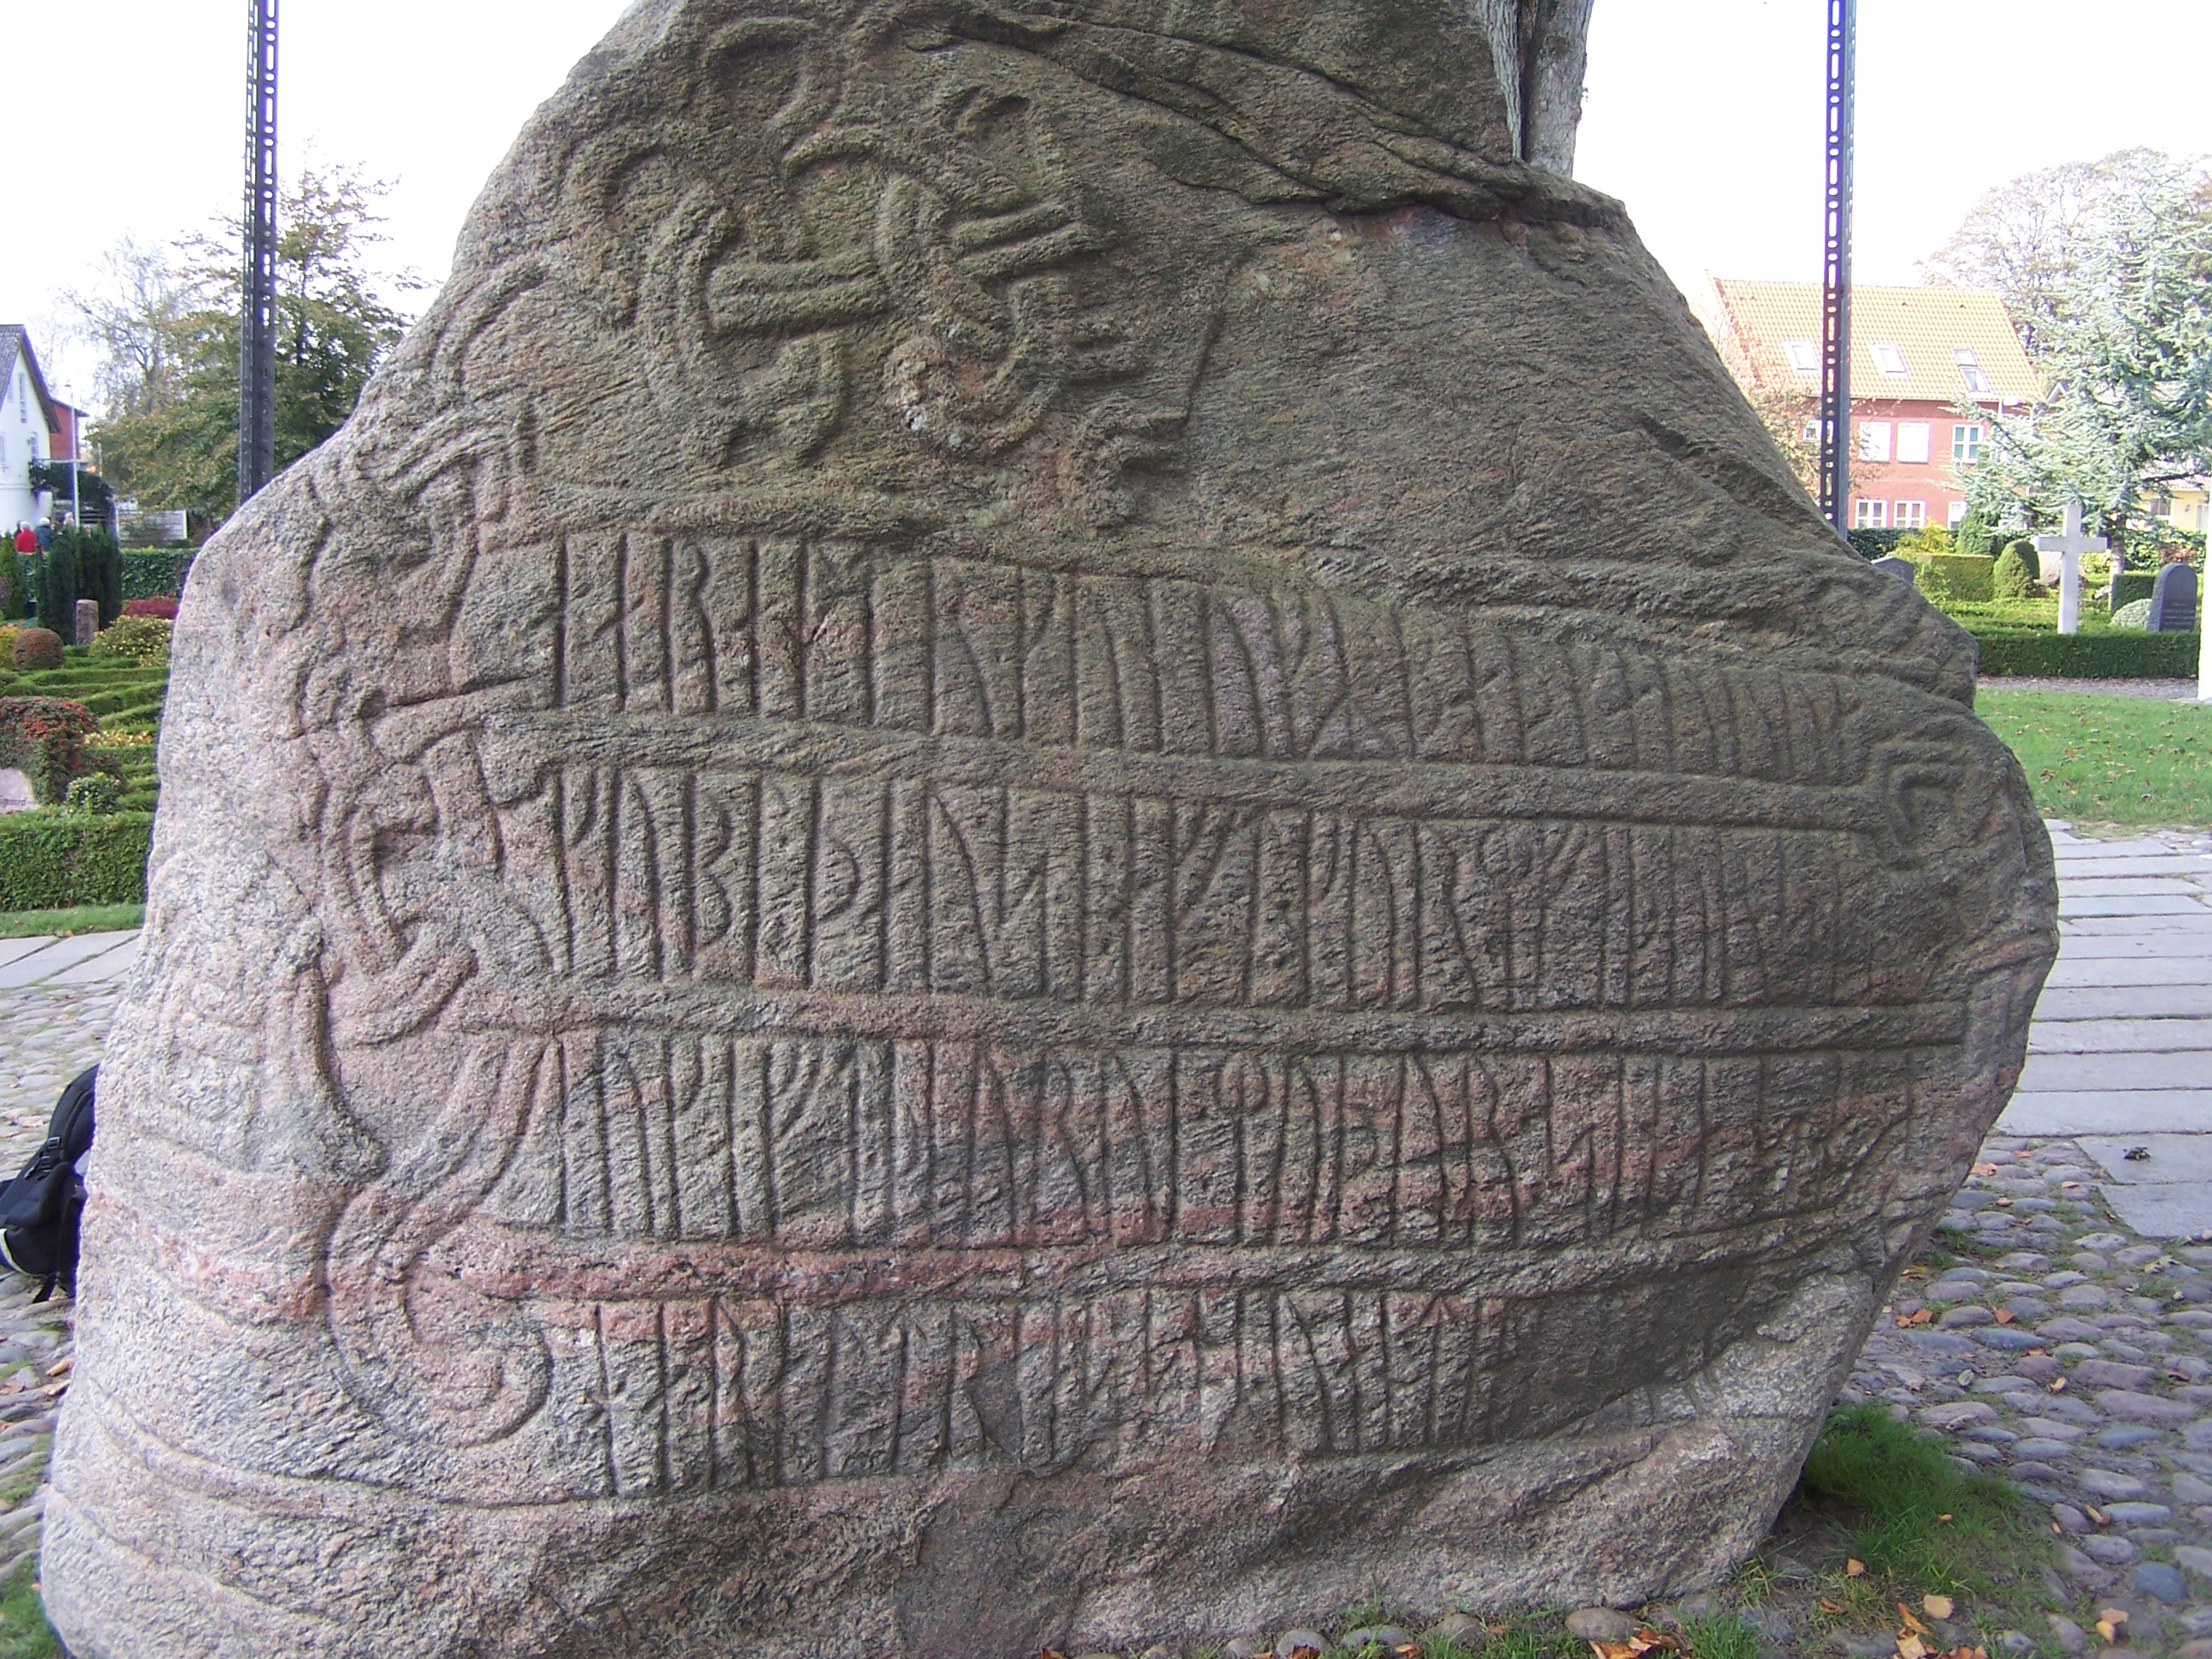
\includegraphics[height=\paperheight,width=\paperwidth]{img/JellingStoneTextside.jpg}};
}

\frame{\titlepage}

\usebackgroundtemplate{}

\begin{frame}
  \frametitle{The first computers were not this}

  \begin{center}
    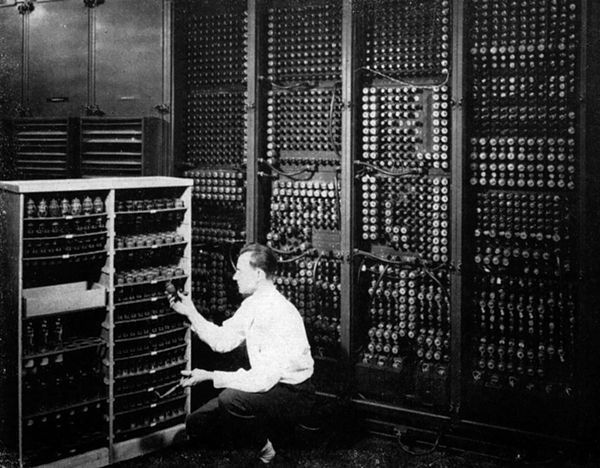
\includegraphics[width=\textwidth]{img/eniac.jpg}
  \end{center}

\end{frame}

\begin{frame}
  \frametitle{But this}

  
\includegraphics[width=\textwidth]{img/human-computer.jpg}
\end{frame}

\begin{frame}
  \frametitle{And if you had a larger problem}

  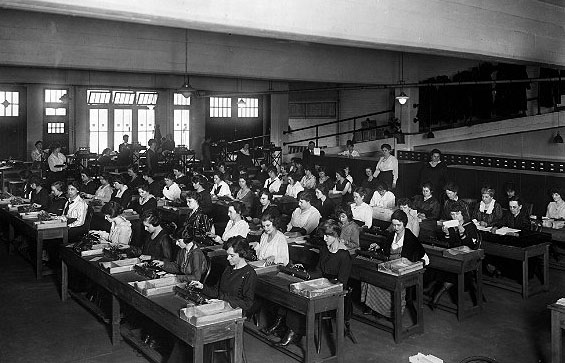
\includegraphics[width=\textwidth]{img/human-computers.jpg}
\end{frame}

\begin{frame}
  \frametitle{But then they started looking like this}

  \begin{center}
    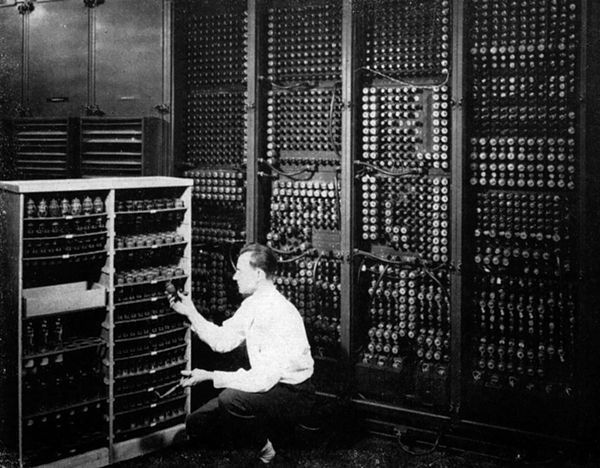
\includegraphics[width=\textwidth]{img/eniac.jpg}
  \end{center}
\end{frame}

\begin{frame}
  \frametitle{Then this}
  \begin{center}
    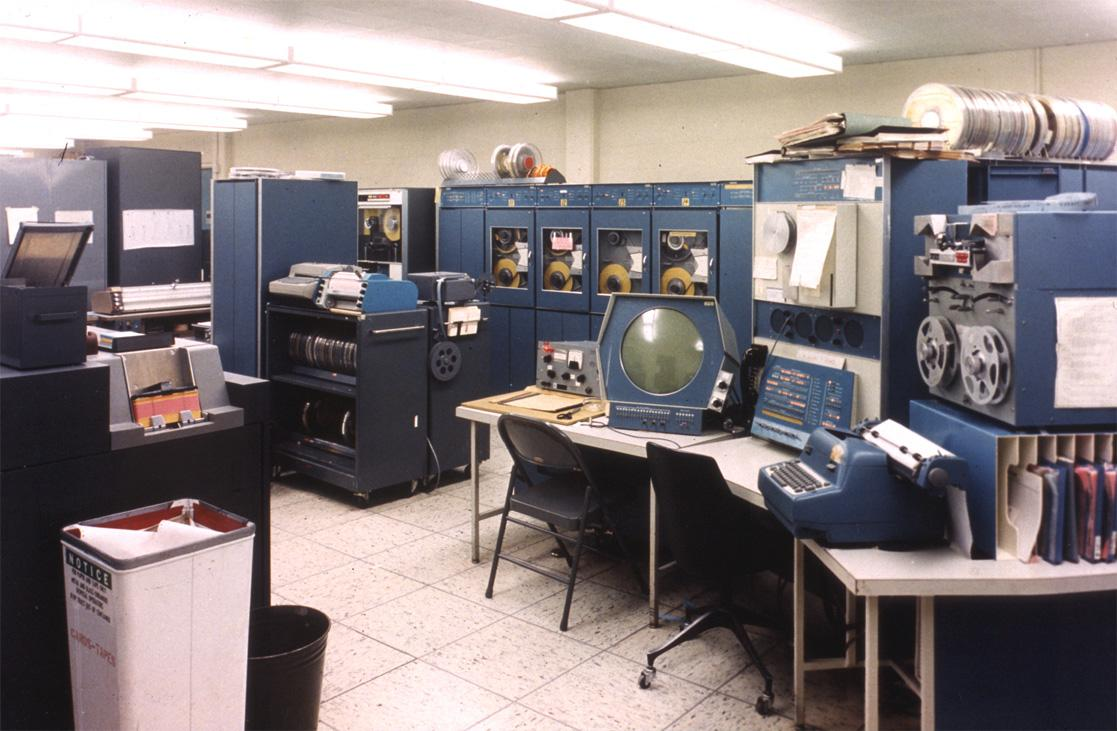
\includegraphics[width=\textwidth]{img/pdp1.jpg}
  \end{center}
\end{frame}

\begin{frame}
  \frametitle{Then this}
  \begin{center}
    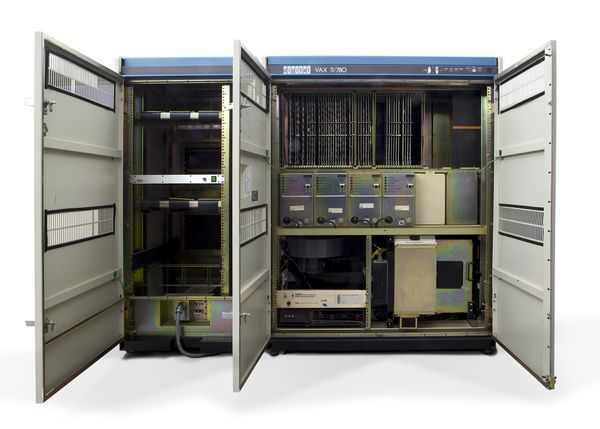
\includegraphics[width=\textwidth]{img/vax.jpg}
  \end{center}
\end{frame}

\begin{frame}
  \frametitle{Then this}
  \begin{center}
    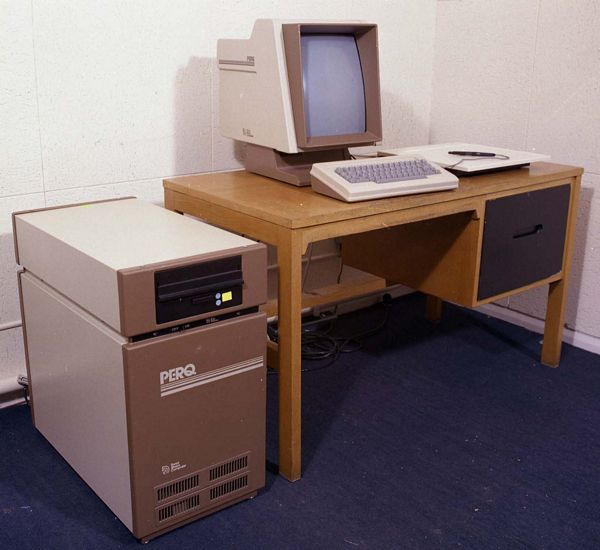
\includegraphics[width=\textwidth]{img/early-workstation.jpg}
  \end{center}
\end{frame}

\begin{frame}
  \frametitle{Then this}
  \begin{center}
    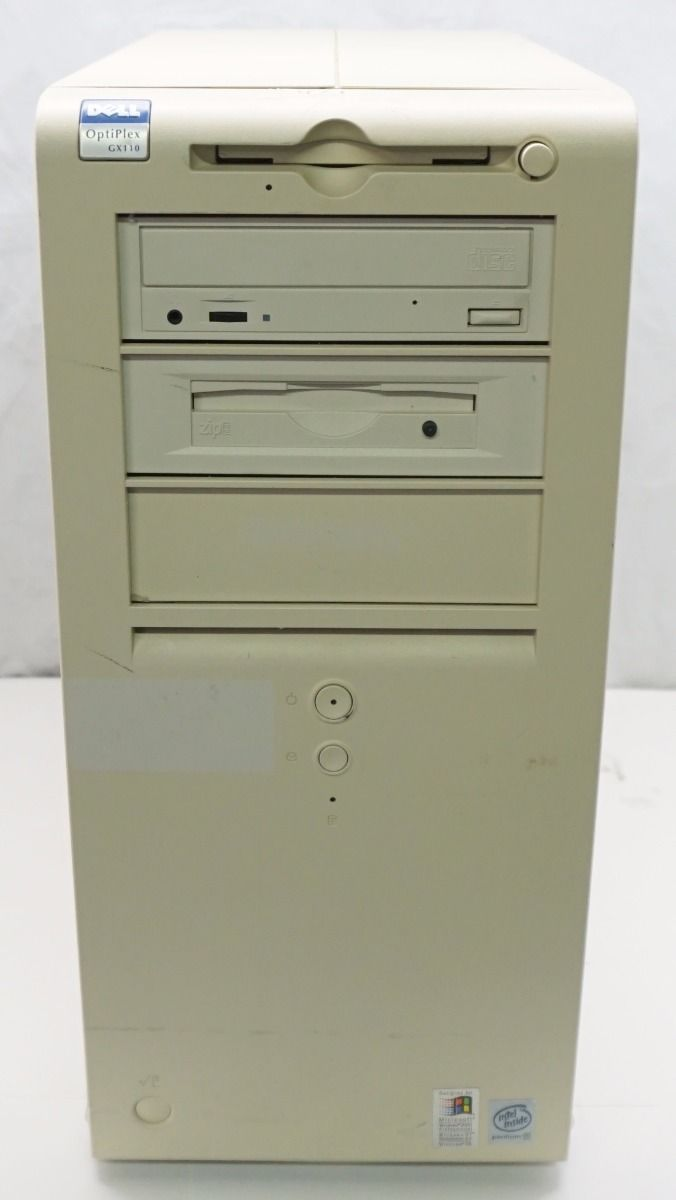
\includegraphics[width=\textwidth]{img/dell.jpg}
  \end{center}
\end{frame}

\begin{frame}
  \frametitle{Then this}
  \begin{center}
    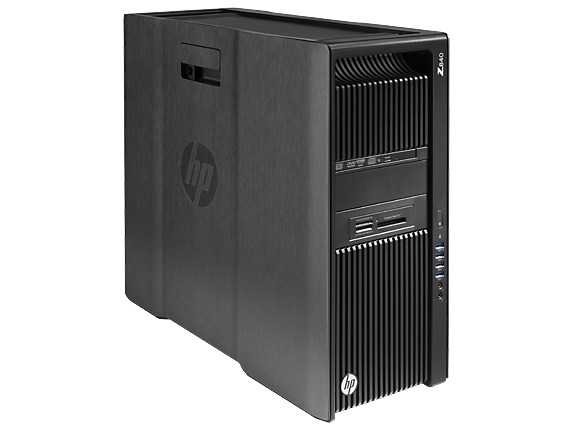
\includegraphics[width=\textwidth]{img/hp.jpg}
  \end{center}
\end{frame}

\begin{frame}
  \frametitle{Then, from around 2005}
  \begin{center}
    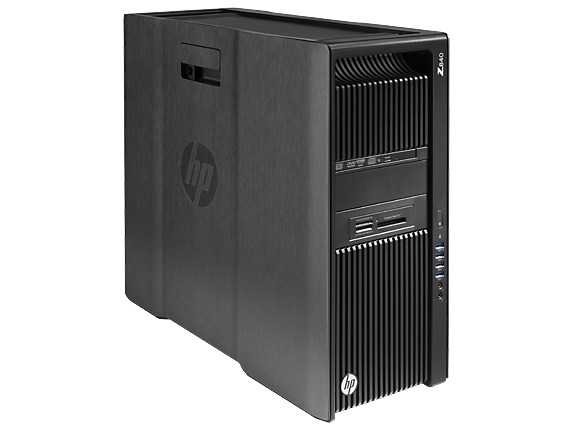
\includegraphics[width=0.5\textwidth]{img/hp.jpg}
    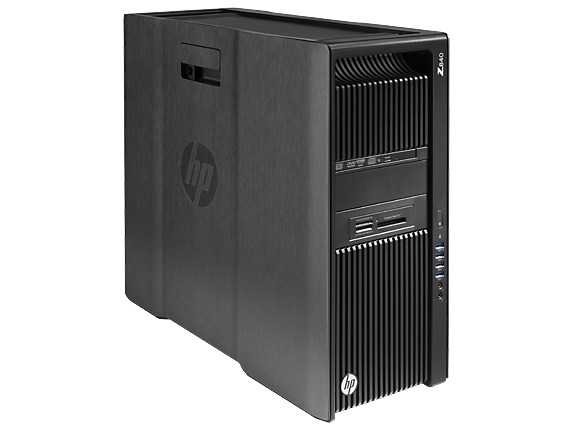
\includegraphics[width=0.5\textwidth]{img/hp.jpg}
  \end{center}
\end{frame}

\begin{frame}
  \frametitle{Then, from around 2005}
  \begin{center}
    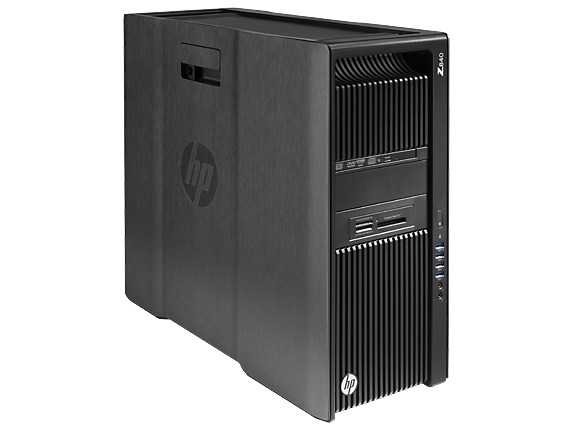
\includegraphics[width=0.3\textwidth]{img/hp.jpg}
    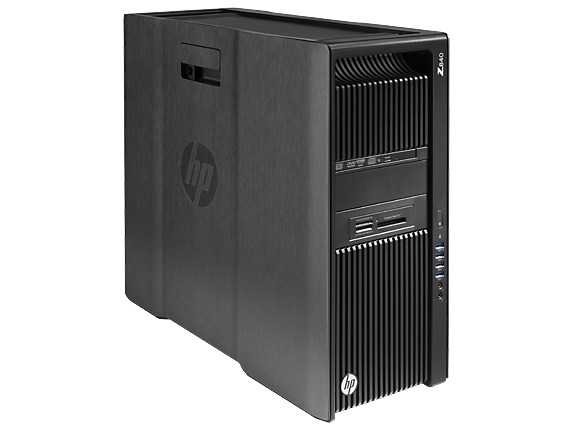
\includegraphics[width=0.3\textwidth]{img/hp.jpg}
    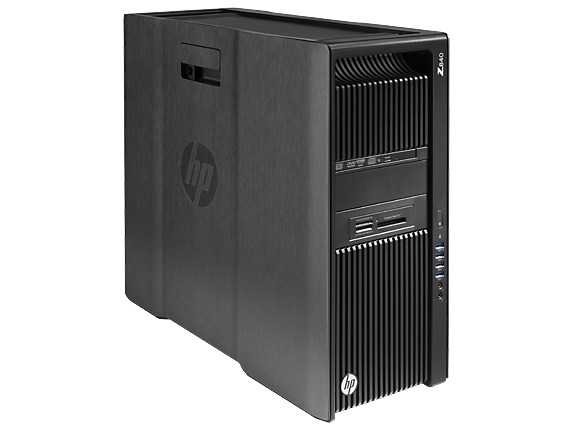
\includegraphics[width=0.3\textwidth]{img/hp.jpg}
  \end{center}

\end{frame}

\begin{frame}
  \frametitle{Then, from around 2005}
  \begin{center}
    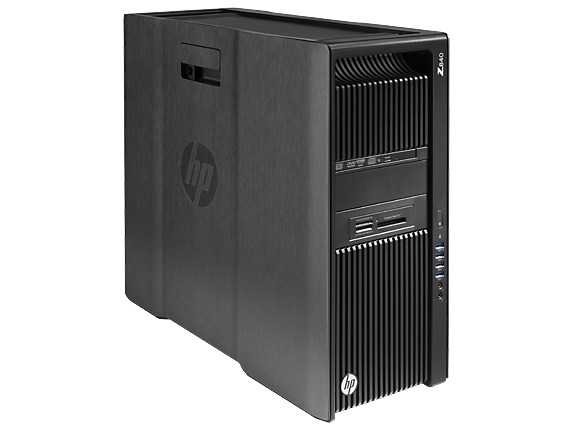
\includegraphics[width=0.3\textwidth]{img/hp.jpg}
    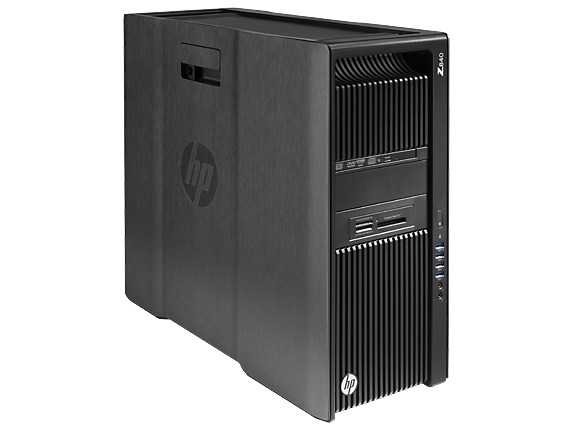
\includegraphics[width=0.3\textwidth]{img/hp.jpg}
    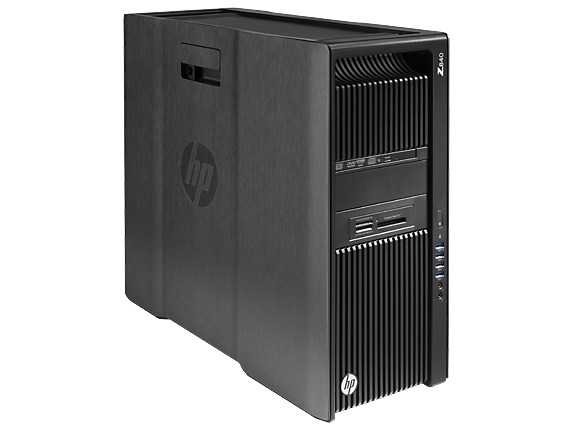
\includegraphics[width=0.3\textwidth]{img/hp.jpg}

    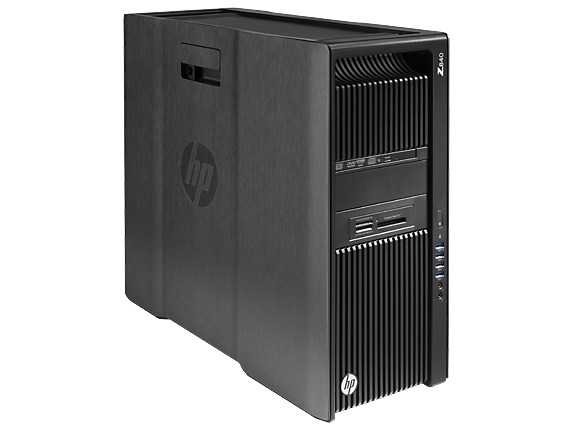
\includegraphics[width=0.3\textwidth]{img/hp.jpg}
    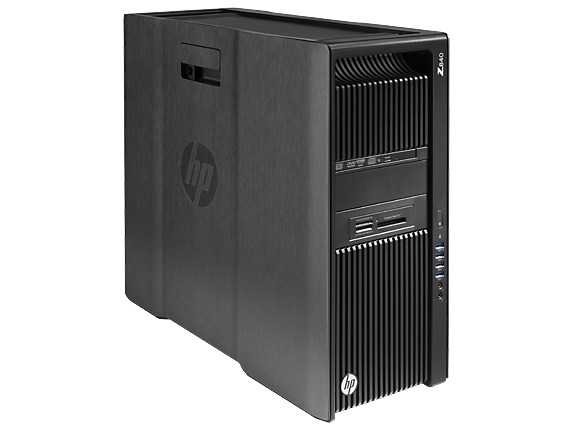
\includegraphics[width=0.3\textwidth]{img/hp.jpg}
    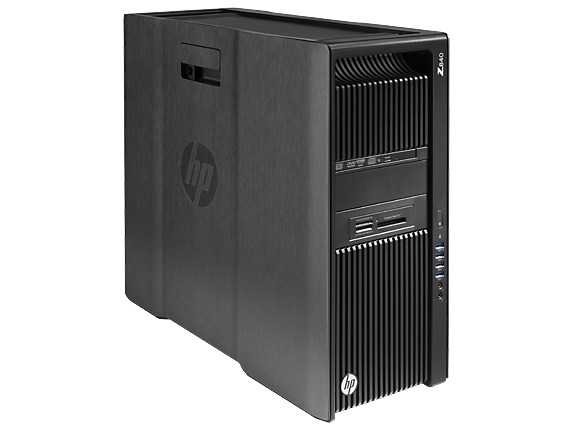
\includegraphics[width=0.3\textwidth]{img/hp.jpg}
  \end{center}

  Improvements in \textit{sequential performance} stalled, although
  computers still got smaller and faster.
\end{frame}


\begin{frame}
  \frametitle{A graph of CPU progress}

  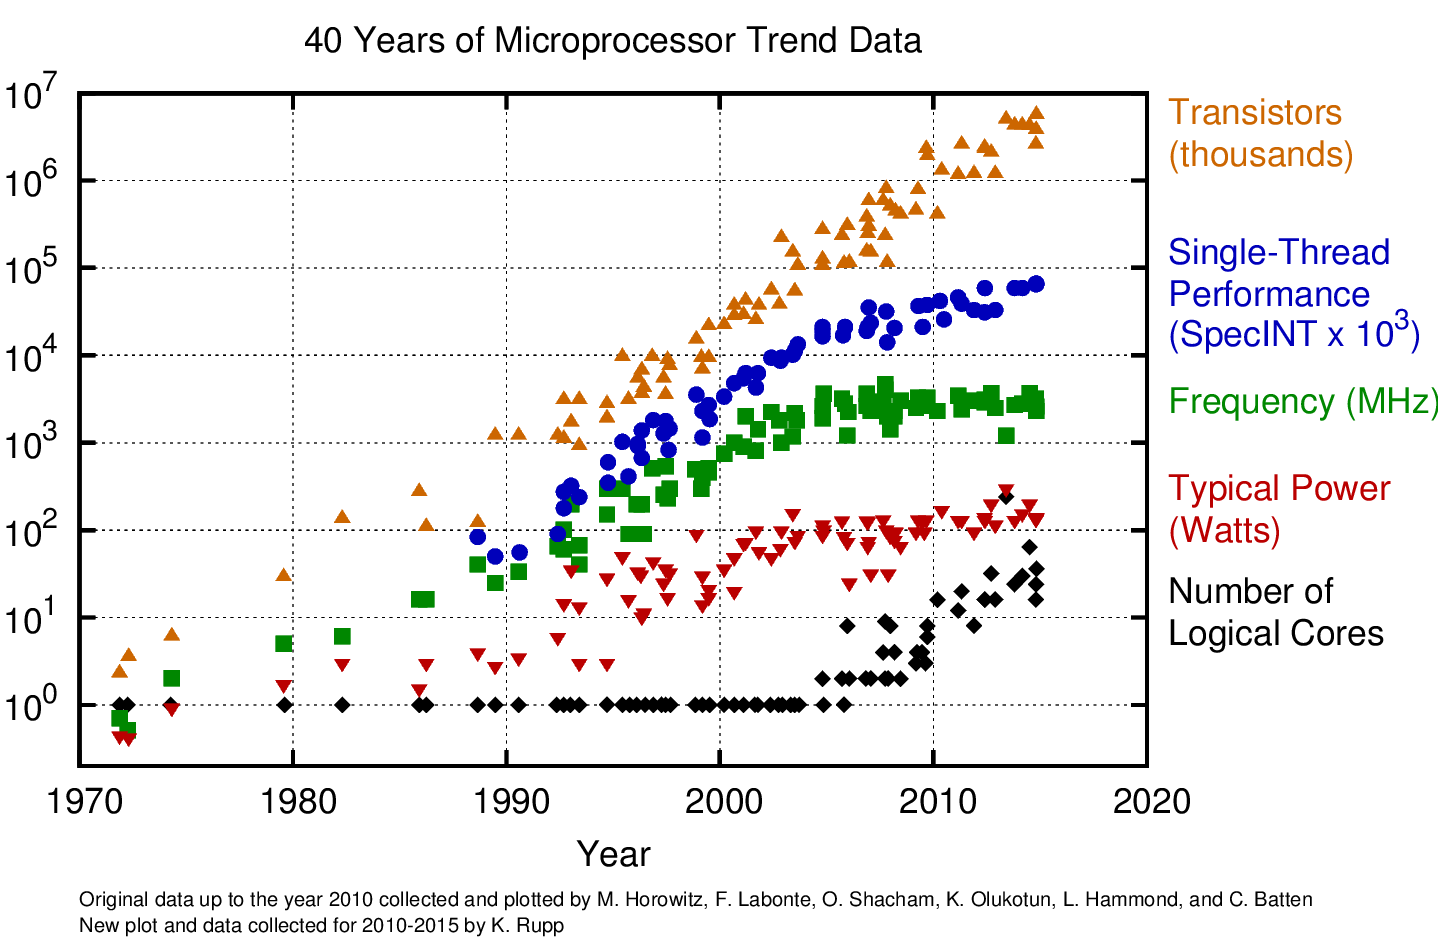
\includegraphics[width=\textwidth]{img/40-years-processor-trend.png}

\end{frame}

\begin{frame}
  \frametitle{The Situation}

  \begin{itemize}
  \item Transistors continue to shrink, so we can continue to build
    ever more advanced computers.
  \item CPU clock speed stalled around 3GHz in 2005, and improvements
    in sequential performance has been slow since then.
  \item Computers still get \textit{faster}, but mostly for parallel
    code.
  \item General-purpose programming now often done on
    \textit{massively parallel} processors, like Graphics Processing
    Units (GPUs).
  \end{itemize}

\end{frame}

\begin{frame}
  \frametitle{GPUs vs CPUs}

  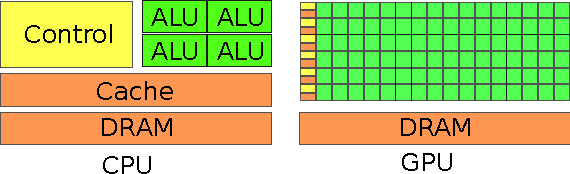
\includegraphics[width=\textwidth]{img/cpu-gpu-architecture.pdf}

  \begin{itemize}
  \item GPUs have \textit{thousands} of simple cores and taking full
    advantage of their compute power requires \textit{tens of
      thousands} of threads.
  \item GPU threads are very \textit{restricted} in what they can do:
    no stack, no allocation, limited control flow, etc.
  \item Potential \textit{very high performance} and \textit{lower
      power usage} compared to CPUs, but programming them is
    \textit{hard}.
  \end{itemize}

  \textbf{Massively parallel processing is currently a special case,
    but will be the common case in the future.}
\end{frame}

\begin{frame}
  \frametitle{Two Guiding Quotes}

  \begin{quote}
    When we had no computers, we had no programming problem
    either. When we had a few computers, we had a mild programming
    problem. Confronted with machines a million times as powerful, we
    are faced with a gigantic programming problem.\\\hfill ---Edsger
    W. Dijkstra (EWD963, 1986)
  \end{quote}

  \pause

  \begin{quote}
    The competent programmer is fully aware of the strictly limited
    size of his own skull; therefore he approaches the programming
    task in full humility, and among other things he avoids clever
    tricks like the plague.\\\hfill ---Edsger W. Dijkstra (EWD340, 1972)
  \end{quote}

\end{frame}

\begin{frame}
  \frametitle{Human brains simply cannot reason about concurrency on a massive scale}

  \begin{itemize}
    \item We need a programming model with \textit{sequential}
      semantics, but that can be \textit{executed} in parallel.
    \item It must be \textit{portable}, because hardware continues to
      change.
    \item It must support \textit{modular} programming.
  \end{itemize}

\end{frame}

\begin{frame}[fragile]
  \frametitle{Sequential Programming for Parallel Machines}

  One approach: write imperative code like we've always done, and
  apply a \textit{parallelising compiler} to try to figure out whether
  parallel execution is possible:

\begin{verbatim}
for (int i = 0; i < n; i++) {
  ys[i] = f(xs[i]);
}
\end{verbatim}

  Is this parallel?  \textbf{Yes.}  But it requires careful inspection
  of read/write indices.
\end{frame}


\begin{frame}[fragile]
  \frametitle{Sequential Programming for Parallel Machines}

  What about this one?

\begin{verbatim}
for (int i = 0; i < n; i++) {
  ys[i+1] = f(ys[i], xs[i]);
}
\end{verbatim}

  \textbf{Yes, but hard for a compiler to detect.}

  \begin{itemize}
  \item Many algorithms are innately parallel, but phrased
    sequentially when we encode them in current languages.
  \item A \textit{parallelising compiler} tries to reverse engineer
    the original parallelism from a sequential formulation.
  \item Possible in theory, is called \textit{heroic effort} for a
    reason.
  \end{itemize}

Why not use a language where we can just say exactly what we mean?

\end{frame}

\begin{frame}[fragile]
  \frametitle{Functional Programming for Parallel Machines}

  Common purely functional combinators have \textit{sequential
    semantics}, but permit \textit{parallel execution}.

  \begin{tabular}{p{0.4\linewidth}p{0.03\linewidth}p{0.49\linewidth}}
\begin{verbatim}
for (int i = 0;
     i < n;
     i++) {
  ys[i] = f(xs[i]);
}
\end{verbatim}
    & \vspace{0.4cm}$\sim$ &
\begin{verbatim}
let ys = map f xs
\end{verbatim}
    \\\hline
\begin{verbatim}
for (int i = 0;
     i < n;
     i++) {
  ys[i+1] = f(ys[i], xs[i]);
}
\end{verbatim}
    & \vspace{0.4cm} $\sim$ &
\begin{verbatim}
let ys = scan f xs
\end{verbatim}
    \\
  \end{tabular}
\end{frame}

\begin{frame}
  \frametitle{Why This Was Worth a PhD Project}

  \begin{description}
  \item[\textbf{Problem:}] Turns out purely functional languages are
    really slow when compiled naively, and GPUs only support certain
    restricted forms of parallelism anyway.

  \pause\item[\textbf{Solution:}] Spend four years co-designing a simple
    language and a non-simple optimising compiler capable of compiling
    it to efficient GPU code: \textbf{Futhark!}
  \end{description}
\end{frame}

\begin{frame}
  \frametitle{Futhark is a high-level language!}

  \begin{itemize}
  \item Futhark is \textit{not} a ``GPU language''---it is a
    hardware-agnostic parallel language.
  \item However, we have written a Futhark \textit{compiler} that can
    generate good GPU code.
  \item The compiler is \textit{not} a ``parallelising compiler''.
    The parallelism is \textit{explicitly given} by the programmer.
    The compiler's job is to figure out what to do with it.  It's more
    of a \textit{sequentialising compiler}.
  \item \textit{Co-design} between compiler and language, inspired by
    hand-written code for target hardware.
  \item GPUs are a challenging target, so if Futhark can be translated
    to good GPU code, then it can probably also be translated to good
    CPU code.
  \end{itemize}

  \textbf{I will talk about key language properties and compilation
    techniques for generating good GPU code.}
\end{frame}


\begin{frame}[fragile]
  \frametitle{Futhark at a Glance}

  Small eagerly evaluated pure functional language with data-parallel
  constructs.  Syntax is a combination of C, SML, and Haskell.

  \begin{itemize}
  \item\textbf{Data-parallel loops}
\begin{lstlisting}[xleftmargin=-1cm]
let add_two [n] (a:  [n]i32):    [n]i32 = map (+2) a
let     sum [n] (a:  [n]i32):       i32 = reduce (+) 0 a
let sumrows [n] (as: [n][m]i32): [n]i32 = map sum as
\end{lstlisting}

  \item\textbf{Array construction}
\begin{lstlisting}[xleftmargin=-1cm]
iota 5           =        [0,1,2,3,4]
replicate 3 1337 = [1337, 1337, 1337]
\end{lstlisting}

    \hfill ---Only regular arrays: \lstinline{[[1,2], [3]]} is illegal.

\item\textbf{Sequential loops}
  \begin{lstlisting}[xleftmargin=-1cm]
loop x = 1 for i < n do
  x * (i + 1)
\end{lstlisting}
  \end{itemize}
\end{frame}

\begin{frame}
  \begin{center}
    \Huge
    CASE STUDY:\\$k$-MEANS CLUSTERING\\
  \end{center}

  \vfill

  \begin{quote}
    Let's do it.\\\hfill---Sonic the Hedgehog (Sonic Rush, 2005)
  \end{quote}
\end{frame}

\begin{frame}
  \frametitle{The Problem}

  We are given $n$ points in some $d$-dimensional space, which we must
  partition into $k$ disjoint sets, such that we minimise the
  inter-cluster sum of squares (the distance from every point in a
  cluster to the centre of the cluster).

  Example with $d=2, k=3, n=\textit{more than I can count}$:

  \begin{center}
    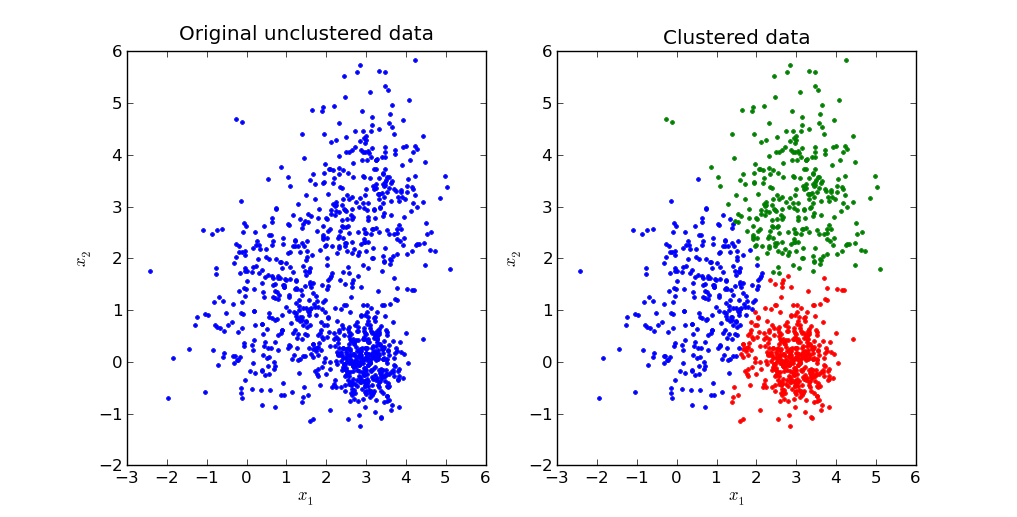
\includegraphics[width=50ex]{img/kmeans.png}
  \end{center}
\end{frame}

\begin{frame}
  \frametitle{The Solution (from Wikipedia)}
  \footnotesize
  \begin{tabular}{p{5cm}p{5cm}}
    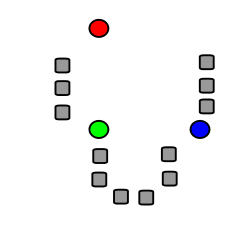
\includegraphics[width=3cm]{img/kmeans1.png} & 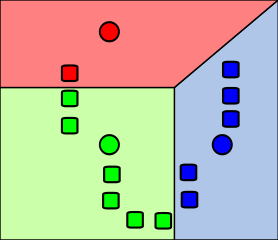
\includegraphics[width=3cm]{img/kmeans2.png} \\

    (1) $k$ initial "means" (here $k=3$) are randomly generated within the data domain. &

    (2) $k$ clusters are created by associating every observation with the nearest mean.\\

    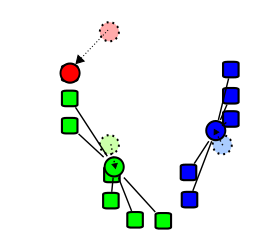
\includegraphics[width=3cm]{img/kmeans3.png} & 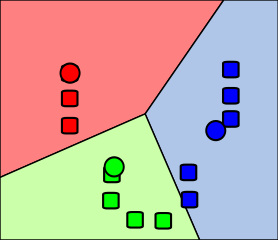
\includegraphics[width=3cm]{img/kmeans4.png} \\

    (3) The centroid of each of the $k$ clusters becomes the new mean. &

    (4) Steps (2) and (3) are repeated until convergence has been reached.
  \end{tabular}
\end{frame}

\begin{frame}[fragile]
  \frametitle{Computing Cluster Means: Fully Sequential}

  \begin{center}
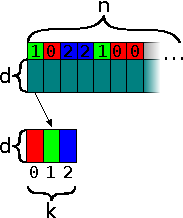
\includegraphics[width=0.6\textwidth]{img/cluster_means_seq_0.pdf}
\end{center}
\end{frame}

\begin{frame}[fragile]
  \frametitle{Computing Cluster Means: Fully Sequential}

  \begin{center}
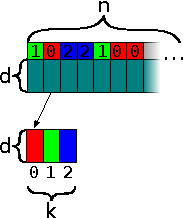
\includegraphics[width=0.6\textwidth]{img/cluster_means_seq_1.pdf}
\end{center}
\end{frame}

\begin{frame}[fragile]
  \frametitle{Computing Cluster Means: Fully Sequential}

  \begin{center}
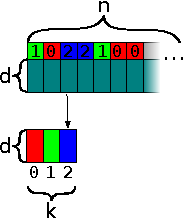
\includegraphics[width=0.6\textwidth]{img/cluster_means_seq_2.pdf}
\end{center}
\end{frame}

\begin{frame}[fragile]
  \frametitle{Computing Cluster Means: Fully Sequential}

  \begin{center}
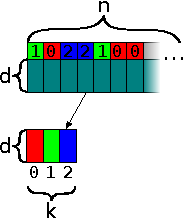
\includegraphics[width=0.6\textwidth]{img/cluster_means_seq_3.pdf}
\end{center}

\end{frame}

\begin{frame}[fragile]
  \frametitle{Computing Cluster Means: Fully Sequential}

\begin{lstlisting}
let add_points [d] (x: [d]f32) (y: [d]f32): [d]f32 =
  map (+) x y

let cluster_means_seq [k][n][d]
                      (cluster_sizes: [k]i32)
                      (points: [n][d]f32)
                      (membership: [n]i32): [k][d]f32 =
  loop acc = replicate k (replicate d 0.0) for i < n do
    let p = points[i]
    let c = membership[i]
    let p' = map (/f32(cluster_sizes[c])) p
    in acc with [c] <- add_points acc[c] p'
\end{lstlisting}
\pause
  \begin{block}{Problem}
    $O(n\times{}d)$ work, but not much parallelism.
  \end{block}

\end{frame}

\begin{frame}[fragile]
  \frametitle{Computing Cluster Means: Fully Parallel}

  \begin{center}
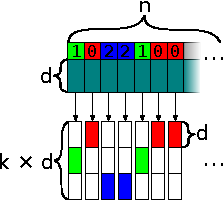
\includegraphics[width=0.8\textwidth]{img/cluster_means_par_0.pdf}
\end{center}
\end{frame}

\begin{frame}[fragile]
  \frametitle{Computing Cluster Means: Fully Parallel}

  \begin{center}
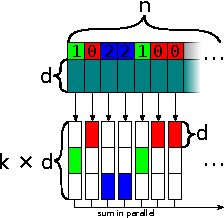
\includegraphics[width=0.8\textwidth]{img/cluster_means_par_1.pdf}
\end{center}
\end{frame}

\begin{frame}[fragile]
  \frametitle{Computing Cluster Means: Fully Parallel}

  Use a parallel \texttt{map} to compute ``increments'', and then a
  \texttt{reduce} of these increments.

\begin{lstlisting}
let matrix_add [k][d]
               (xss: [k][d]f32) (yss: [k][d]f32): [k][d]f32 =
  map (\xs ys -> map (+) xs ys) xss yss

let cluster_means_par [k][n][d]
                      (cluster_sizes: [k]i32)
                      (points: [n][d]f32)
                      (membership: [n]i32): [k][d]f32 =
  let increments : [n][k][d]i32 =
    map (\p c -> let a = replicate k (replicate d 0.0)
                let p' = map (/(f32(cluster_sizes[c]))) p
                in a with [c] <- p')
        points membership
  in reduce matrix_add (replicate k (replicate d 0.0))
            increments

\end{lstlisting}
\pause
  \begin{block}{Problem}
    Fully parallel, but $O(k\times{}n\times{}d)$ work.
  \end{block}
\end{frame}

\begin{frame}
  \frametitle{One Futhark Design Principle}

  \begin{block}{}
    The hardware is not infinitely parallel - ideally, we use an
    efficient sequential algorithm for chunks of the input, then use a
    parallel operation to combine the results of the sequential parts.
  \end{block}

  \begin{center}
    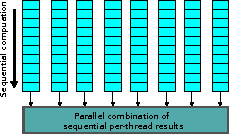
\includegraphics[width=7cm]{img/chunking.pdf}
  \end{center}

  The optimal number of threads varies from case to case, so this
  should be abstracted from the programmer.
\end{frame}

\begin{frame}[fragile]
  \frametitle{Computing Cluster Means: Just Right}

  \begin{center}
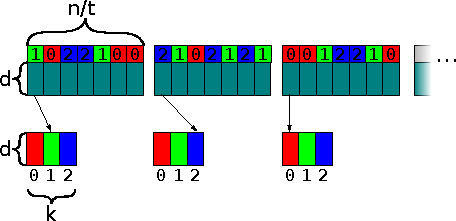
\includegraphics[width=\textwidth]{img/cluster_means_chunked_0.pdf}
\end{center}
\end{frame}

\begin{frame}[fragile]
  \frametitle{Computing Cluster Means: Just Right}

  \begin{center}
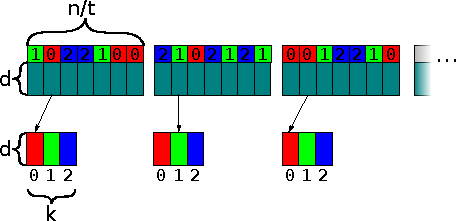
\includegraphics[width=\textwidth]{img/cluster_means_chunked_1.pdf}
\end{center}
\end{frame}

\begin{frame}[fragile]
  \frametitle{Computing Cluster Means: Just Right}

  \begin{center}
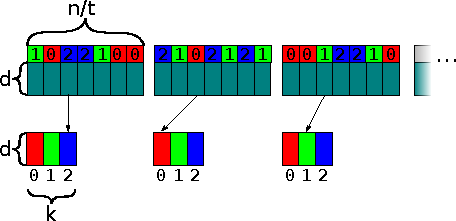
\includegraphics[width=\textwidth]{img/cluster_means_chunked_2.pdf}
\end{center}
\end{frame}

\begin{frame}[fragile]
  \frametitle{Computing Cluster Means: Just Right}

  \begin{center}
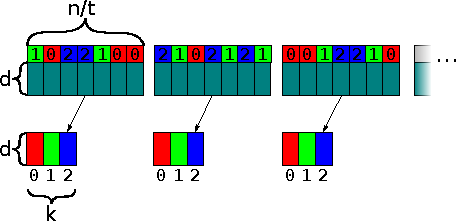
\includegraphics[width=\textwidth]{img/cluster_means_chunked_3.pdf}
\end{center}
\end{frame}

\begin{frame}[fragile]
  \frametitle{Computing Cluster Means: Just Right}

  \begin{center}
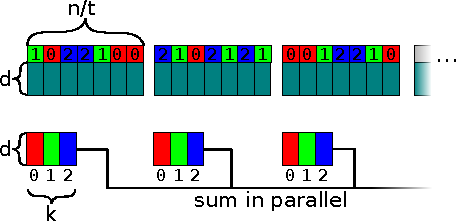
\includegraphics[width=\textwidth]{img/cluster_means_chunked_reduce.pdf}
\end{center}
\end{frame}

\begin{frame}[fragile]
  \frametitle{Computing Cluster Sizes: Just Right}

  We use a Futhark language construct called a \textit{stream
    reduction}.

  \begin{lstlisting}
let cluster_means_stream [k][n][d]
                         (cluster_sizes: [k]i32)
                         (points: [n][d]f32)
                         (membership: [n]i32): [k][d]f32 =
  stream_red
    matrix_add
    (\[chunk_size]
      (points':     [chunk_size][d]f32)
      (membership': [chunk_size]i32) ->
        cluster_means_seq cluster_sizes points' membership')
    points membership
\end{lstlisting}

  \begin{description}
  \item[\textbf{For full parallelism},] set chunk size to $1$.
  \item[\textbf{For full sequentialisation},] set chunk size to \texttt{n}.
  \end{description}

\end{frame}

\begin{frame}[fragile]
  \frametitle{GPU Code Generation for \texttt{stream\_red}}

  Broken up as:

  \begin{lstlisting}
let per_thread_results : [num_threads][k][d]f32 =
  ...
-- combine the per-thread results
let cluster_means =
  reduce (map (map (+)))
         (replicate k (replicate d 0.0))
         per_thread_results
\end{lstlisting}

  The reduction with \lstinline{map (map (+))} is not great, as
  parallelism inside of a reduction operator cannot be exploited.

  The compiler will recognise this structure and perform a
  transformation called \textit{Interchange Reduce With Inner Map}
  (IRWIM); moving the reduction inwards at a cost of a transposition.
\end{frame}

\begin{frame}[fragile]
  \frametitle{After IRWIM}

  We transform
  \begin{lstlisting}
let cluster_means =
  reduce (map (map (+)))
         (replicate k (replicate d 0.0))
         per_thread_results
\end{lstlisting}

and get

\begin{lstlisting}
let per_thread_results' : [k][d][num_threads]f32 =
  !rearrange (1,2,0)! per_thread_results
let cluster_sizes =
  map (map (reduce (+) 0.0)) per_thread_results'
\end{lstlisting}

\begin{itemize}
\item \lstinline{map} parallelism of size $\texttt{k}\times\texttt{d}$ -
  likely not enough.
\item The Futhark compiler generates a \textit{segmented reduction}
  for
  \lstinline{map (map (reduce (+) 0.0))}, which exploits also the
  innermost \lstinline{reduce} parallelism.
\end{itemize}
\end{frame}

\begin{frame}
  \frametitle{Speedup on GPU of Chunked vs. Fully Parallel Implementation}

  \begin{itemize}
  \item \textbf{Hardware}: \hfill NVIDIA Tesla K40
  \item \textbf{Input}: \hfill $k=5$; $n=10,000,000$; $d=3$.
  \item \textbf{Fully parallel runtime:} \hfill 134.1ms
  \item \textbf{Chunked runtime:} \hfill 17.6ms
  \end{itemize}

  \vspace{2cm}
  \centering\large Speedup: $\times7.6$
\end{frame}

\begin{frame}
  \begin{center}
    \Huge IMPROVING AVAILABLE PARALLELISM VIA LOOP DISTRIBUTION AND INTERCHANGE
  \end{center}

\vfill
  \begin{quote}
    Oh, look! It changed shape! Did you see that?! \\\hfill ---Miles ``Tails'' Prower (Sonic Adventure, 1998)
  \end{quote}
\end{frame}

\begin{frame}[fragile]
  \frametitle{The Problem}

  Futhark permits \textit{nested} (regular) parallelism, but GPUs
  prefer \textit{flat} parallel \textit{kernels}.

  \pause \vspace{1cm} \textbf{Solution:} Have the compiler rewrite
  program to perfectly nested \lstinline{map}s containing sequential
  code (or known parallel patterns such as segmented reduction), each
  of which can become a GPU kernel.  \pause
\begin{center}
\begin{tabular}{c}
\begin{lstlisting}
map (\xs -> let y = reduce (+) 0 xs
           in map (+y) xs)
    xss
\end{lstlisting}
\end{tabular}

  $\Downarrow$

\begin{tabular}{c}
\begin{lstlisting}
let ys = map (\xs -> reduce (+) 0 xs) xss
in map (\xs y -> map (+y) xs) xss ys
\end{lstlisting}
\end{tabular}
\end{center}
\end{frame}

\begin{frame}
  \frametitle{The Universal Approach: Full Flattening}

  \begin{itemize}
  \item Developed by Guy Blelloch in the early 90s.
  \item Able to exploit \textit{all} parallelism.
  \item Always maximises parallelism, even when not worthwhile (e.g
    innermost loops in a matrix multiplication).
  \item Wasteful of memory (fully flattened matrix multiplication
    requires $O(n^{3})$ space).
  \item Destroys access pattern information, rendering
    locality-of-reference optimisations hard or impossible.
  \end{itemize}

  We want to exploit the parallelism that is \textit{profitable}, but
  not more.

\end{frame}

\begin{frame}
  \frametitle{Limited Flattening via Loop Fission}

  The classic map fusion rule:

  \[
    \text{map}~f \circ \text{map}~g \Rightarrow \text{map}~(f \circ g)
  \]

\vspace{1cm}
\pause
We can also apply it backwards to obtain \textit{fission}:

  \[
     \text{map}~(f \circ g) \Rightarrow \text{map}~f \circ \text{map}~g
  \]

  This, along with other higher-order rules (see thesis), are applied
  by the compiler to extract perfect map nests.

\end{frame}

\begin{frame}[t,fragile]
\frametitle{Example: (a) Initial program, we inspect the map-nest.}

  \begin{lstlisting}[basicstyle=\sffamily\footnotesize]
let (asss, bss) =
  map (\(ps: [m]i32) ->
        let ass = map (\(p: i32): [m]i32 ->
                        let cs = scan (+) 0 (iota p)
                        let r = reduce (+) 0 cs
                        in map (+r) ps) ps
        @let bs = loop ws=ps for i < n do
                    map (\as w: i32 ->
                          let d = reduce (+) 0 as
                          let e = d + w
                          in 2 * e) ass ws@
        in (ass, bs)) pss
\end{lstlisting}

We assume the type of \texttt{pss : [m][m]i32}.
\end{frame}

\begin{frame}[t,fragile]
\frametitle{(b) Distribution.}

\begin{lstlisting}[basicstyle=\sffamily\footnotesize]
let asss: [m][m][m]i32 =
  map (\(ps: [m]i32) ->
        let ass = map (\(p: i32): [m]i32 ->
                        let cs = scan (+) 0 (iota p)
                        let r = reduce (+) 0 cs
                        in map (+r) ps) ps
        in ass) pss
!let bss: [m][m]i32 =
  map (\ps ass ->
        let bs = loop ws=ps for i < n do
                    map (\as w ->
                          let d = reduce (+) 0 as
                          let e = d + w
                          in 2 * e) ass ws
        in bs) pss asss!
\end{lstlisting}
\end{frame}

\begin{frame}[t,fragile]
\frametitle{(c) Interchanging outermost map inwards.}

\begin{lstlisting}[basicstyle=\sffamily\footnotesize]
let asss: [m][m][m]i32 =
  map (\(ps: [m]i32) ->
        let ass = map (\(p: i32): [m]i32 ->
                        let cs = scan (+) 0 (iota p)
                        let r = reduce (+) 0 cs
                        in map (+r) ps) ps
        in ass) pss
let bss: [m][m]i32 =
  map (\ps ass ->
        @let bs = loop ws=ps for i < n do
                    map (\as w ->
                          let d = reduce (+) 0 as
                          let e = d + w
                          in 2 * e) ass ws@
        in bs) pss asss
\end{lstlisting}
\end{frame}


\begin{frame}[t,fragile]
\frametitle{(c) Interchanging outermost map inwards.}

\begin{lstlisting}[basicstyle=\sffamily\footnotesize]
let asss: [m][m][m]i32 =
  map (\(ps: [m]i32) ->
        let ass = map (\(p: i32): [m]i32 ->
                        let cs = scan (+) 0 (iota p)
                        let r = reduce (+) 0 cs
                        in map (+r) ps) ps
        in ass) pss
let bss: [m][m]i32 =!
  loop wss=pss for i < n do
    map (\ass ws ->
          let ws' = map (\as w ->
                          let d = reduce (+) 0 as
                          let e = d + w
                          in 2 * e) ass ws
          in ws') asss wss!
\end{lstlisting}
\end{frame}

\begin{frame}[t,fragile]
\frametitle{(d) Skipping scalar computation.}

\begin{lstlisting}[basicstyle=\sffamily\footnotesize]
let asss: [m][m][m]i32 =
  map (\(ps: [m]i32) ->
        let ass = map (\(p: i32): [m]i32 ->
                        let cs = scan (+) 0 (iota p)
                        let r = reduce (+) 0 cs
                        in map (+r) ps) ps
        in ass) pss
let bss: [m][m]i32 =
  loop wss=pss for i < n do
    map (\ass ws ->
          let ws' = map (\as w ->
                          let d = reduce (+) 0 as
                          let e = d + w
                          @in 2 * e@) ass ws
          in ws') asss wss
\end{lstlisting}
\end{frame}

\begin{frame}[t,fragile]
\frametitle{(d) Skipping scalar computation.}

\begin{lstlisting}[basicstyle=\sffamily\footnotesize]
let asss: [m][m][m]i32 =
  map (\(ps: [m]i32) ->
        let ass = map (\(p: i32): [m]i32 ->
                        let cs = scan (+) 0 (iota p)
                        let r = reduce (+) 0 cs
                        in map (+r) ps) ps
        in ass) pss
let bss: [m][m]i32 =
  loop wss=pss for i < n do
    map (\ass ws ->
          let ws' = map (\as w ->
                          let d = reduce (+) 0 as
                          @let e = d + w@
                          in 2 * e) ass ws
          in ws') asss wss
\end{lstlisting}
\end{frame}

\begin{frame}[t,fragile]
\frametitle{(e) Distributing reduction..}

\begin{lstlisting}[basicstyle=\sffamily\footnotesize]
let asss: [m][m][m]i32 =
  map (\(ps: [m]i32) ->
        let ass = map (\(p: i32): [m]i32 ->
                        let cs = scan (+) 0 (iota p)
                        let r = reduce (+) 0 cs
                        in map (+r) ps) ps
        in ass) pss
let bss: [m][m]i32 =
  loop wss=pss for i < n do
    map (\ass ws ->
          let ws' = map (\as w ->
                          @let d = reduce (+) 0 as@
                          let e = d + w
                          in 2 * e) ass ws
          in ws') asss wss
\end{lstlisting}
\end{frame}

\begin{frame}[t,fragile]
\frametitle{(e) Distributing reduction.}

\begin{lstlisting}[basicstyle=\sffamily\footnotesize]
let asss: [m][m][m]i32 =
  map (\(ps: [m]i32) ->
        let ass = map (\(p: i32): [m]i32 ->
                        let cs = scan (+) 0 (iota p)
                        let r = reduce (+) 0 cs
                        in map (+r) ps) ps
        in ass) pss
let bss: [m][m]i32 =
  loop wss=pss for i < n do
!    let dss: [m][m]i32 =
      map (\ass ->
            map (\as ->
                  reduce (+) 0 as) ass)
          asss!
    in map (\ws !ds! ->
             let ws' =
                map (\w !d! -> let e  = d + w
                            in 2 * e) ws !ds!
             in ws') asss !dss!
\end{lstlisting}
\end{frame}

\begin{frame}[t,fragile]
\frametitle{(f) Distributing inner map.}

\begin{lstlisting}[basicstyle=\sffamily\footnotesize]
let asss =
  map (\(ps: [m]i32) ->
        let ass = map (\(p: i32): [m]i32 ->
                        let cs = scan (+) 0 (iota p)
                        let r = reduce (+) 0 cs
                        @in map (+r) ps) ps@
        in ass) pss
let bss: [m][m]i32 = ...
\end{lstlisting}
\end{frame}

\begin{frame}[t,fragile]
\frametitle{(f) Distributing inner map.}

\begin{lstlisting}[basicstyle=\sffamily\footnotesize]
let !rss: [m][m]i32! =
  map (\(ps: [m]i32) ->
        let !rss! = map (\(p: i32): !i32! ->
                        let cs = scan (+) 0 (iota p)
                        let r = reduce (+) 0 cs
                        in !r!) ps
        in !rss!) pss
let asss: [m][m][m]i32 =!
  map (\(ps: [m]i32) (rs: [m]i32) ->
        map (\(r: i32): [m]i32 ->
              @map (+r) ps) rs@
      ) pss rss!
let bss: [m][m]i32 = ...
\end{lstlisting}
\end{frame}

\begin{frame}[t,fragile]
\frametitle{(g) Cannot distribute as it would create irregular array.}

\begin{lstlisting}[basicstyle=\sffamily\footnotesize]
let rss: [m][m]i32 =
  map (\(ps: [m]i32) ->
        let rss = map (\(p: i32): i32 ->
                        let cs = scan (+) 0 (iota p)
                        let r = @reduce (+) 0 cs@
                        in r) ps
        in rss) pss
let asss: [m][m][m]i32 = ...
let bss: [m][m]i32 = ...
\end{lstlisting}

Array \texttt{cs} has type \texttt{[p]i32}, and \texttt{p} is variant
to the innermost map nest.
\end{frame}

\begin{frame}[t,fragile]
\frametitle{(h) These statements are sequentialised}

\begin{lstlisting}[basicstyle=\sffamily\footnotesize]
let rss: [m][m]i32 =
  map (\(ps: [m]i32) ->
        let rss = map (\(p: i32): i32 ->@
                        let cs = scan (+) 0 (iota p)
                        let r = reduce (+) 0 cs
                        in r@) ps
        in rss) pss
let asss: [m][m][m]i32 = ...
let bss: [m][m]i32 = ...
\end{lstlisting}

Array \texttt{cs} has type \texttt{[p]i32}, and \texttt{p} is variant
to the innermost map nest.
\end{frame}

\begin{frame}[t,fragile]
\frametitle{Result}

\begin{lstlisting}[basicstyle=\sffamily\footnotesize]
let rss: [m][m]i32 = map (\ps -> map (...) ps) pss
let asss: [m][m][m]i32 =
  map (\ps rs -> map (\r -> map (...) ps) rs) pss rss
let bss: [m][m]i32 =
  loop wss=pss for i < n do
    let dss: [m][m]i32 = map (\ass -> map (reduce ...) ass)
                             asss
    in map (\ws ds -> map (...) ws ds ) asss dss
\end{lstlisting}

\vspace{1cm}

From a single kernel with parallelism $m$ to four kernels of
parallelism $m^{2}$, $m^{3}$, $m^{3}$, and
$m^{2}$.

The last two kernels are executed $n$ times each.
\end{frame}

\begin{frame}
  \begin{center}
    \huge EMPIRICAL VALIDATION
  \end{center}
\vfill
  \begin{quote}
    I'll show you what true speed REALLY is! \\\hfill ---Sonic the
    Hedgehog (Sonic Riders, 2006)
  \end{quote}
\end{frame}

\begin{frame}
\frametitle{Empirical validation}

  \textbf{The Question:} Is it possible to construct a purely functional
  hardware-agnostic programming language that is convenient to use and
  provides good parallel performance?

  \textbf{Hard to Prove:} Only performance is easy to quantify, and
  even then...

  \begin{itemize}
  \item No good objective criterion for whether a language is ``fast''.
  \item Best practice is to take benchmark programs written in other
    languages, port or re-implement them, and see how they behave.
  \item Most benchmarks (16) originally written in low-level CUDA or
    OpenCL, but a few (5) are from Accelerate, another high-level
    parallel language.
  \end{itemize}

\end{frame}

\begin{frame}
  \frametitle{Rodinia}

  \begin{minipage}{0.6\linewidth}
    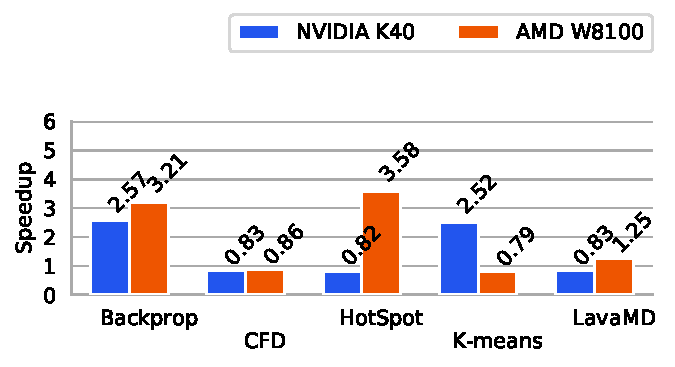
\includegraphics[scale=0.6]{img/rodinia1.pdf}

    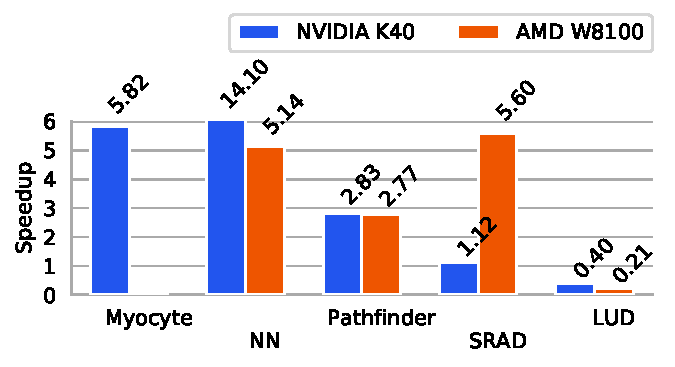
\includegraphics[scale=0.6]{img/rodinia2.pdf}
  \end{minipage}
  \begin{minipage}{0.39\linewidth}
    \begin{itemize}
    \item CUDA and OpenCL implementations of widely varying quality.
    \item This makes them ``realistic'', in a sense.
    \end{itemize}
  \end{minipage}
\end{frame}

\begin{frame}[fragile]
  \frametitle{Rodinia: HotSpot --- a stencil application\\0.82$\times$ ``speedup''}

  At a high level, the stencil is a sequential loop containing a
  nested \lstinline{map} over the $m\times{}m$ iteration space:

\begin{lstlisting}
loop s = s0 for i < n do
  let s' = map (\i -> map (f s i) [0...m-1]) [0...m-1]
  in s'
\end{lstlisting}

  \begin{itemize}
  \item Futhark performs a copy of the intermediate \lstinline{s'} array for
    every iteration, while the reference implementation does pointer swapping.
  \item These copies account for 30\% of runtime; which is why the
    reference implementation is slightly faster.
  \end{itemize}
\end{frame}

\begin{frame}[fragile]
  \frametitle{Rodinia: SRAD --- a stencil application with some
    differential equations\\1.12$\times$ speedup}

Same rough pattern as HotSpot:

\begin{lstlisting}
loop s = s0 for i < n do
  let x = reduce (+) 0 (reshape (m*m) s)
  let s' = map (\i -> map (f s i) [0...m-1]) [0...m-1]
  in s'
\end{lstlisting}

\begin{itemize}
\item But note the reduction!
\item They are tedious to implement efficiently, and the reference
  implementation contains a naive implementation that loses maybe 30\%
  potential performance.
\item The Futhark compiler does not get bored, and performs even the
  tedious optimisations, which is enough to win here.
\item Humans are good at the big picture, and compilers can resolve
  the details --- and they do add up.
\end{itemize}

\end{frame}

\begin{frame}
  \frametitle{Rodinia: LUD}

  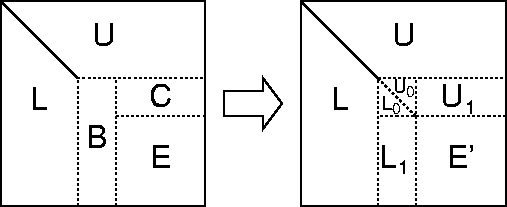
\includegraphics[width=\textwidth]{img/lud.png}

  \bigskip{\small (Illustration from \textit{Software Libraries for
      Linear Algebra Computations on High Performance Computers}, by
    Jack J. Dongarra and David W. Walker.)}

\end{frame}

\begin{frame}[fragile]
  \frametitle{Rodinia: LUD --- computing the block \\ 0.40$\times$ speedup}

  A loop that is roughly

\begin{lstlisting}
map (\x ->
      loop ys=ys0 for i < n do
        map (\y -> ...) ys)
    xs
\end{lstlisting}

  Futhark maps this to GPU code by \textit{interchanging} the outer
  \lstinline{map} inwards:

\begin{lstlisting}
loop yss=yss0 for i < n do
  map (\x ys ->
        map (\y -> ...) ys)
      xs yss
\end{lstlisting}

  Results in $n$ kernel launches, and $n$ stores of intermediate
  results to global memory.

  The Rodinia implementation executes the inner
  \lstinline{map} directly in a GPU group, saving a \textit{lot} of
  overhead.
\end{frame}

\begin{frame}
  \frametitle{Parboil}

  \begin{center}
    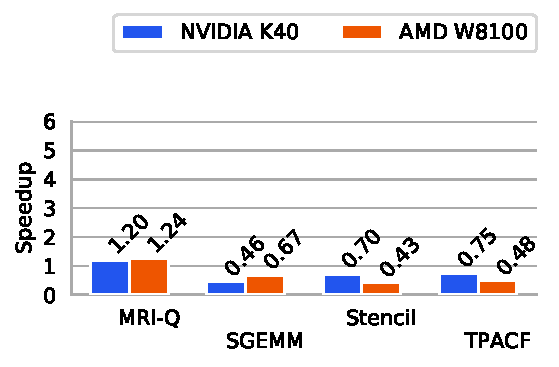
\includegraphics[scale=0.8]{img/parboil.pdf}
  \end{center}


  \begin{itemize}
  \item CUDA and OpenCL implementations of consistently high quality.
  \item That we even get this close is a pretty good result!
  \end{itemize}

\end{frame}

\newcommand{\SGg}{\cellcolor{blue!40}}
\newcommand{\SGgt}{\cellcolor{blue!20}}
\newcommand{\SGt}{\cellcolor{green!30}}
\newcommand{\SGthI}{\cellcolor{blue!65}}
\newcommand{\SGthII}{\cellcolor{blue!75}}
\newcommand{\SGthIII}{\cellcolor{blue!95}}

\begin{frame}
  \frametitle{Parboil: SGEMM --- matrix multiplication \\ 0.46$\times$ speedup}

  \begin{minipage}{0.49\linewidth}
  \begin{tabular}{|c|c|c|c|c|c|c|c|c|c|c|c|c|c|c|c|c|c|}
    \hline
    &&&&&&&\SGt{}&&&&\\\hline
    &&&&&&&\SGt{}&&&&\\\hline
    &&&&&&&\SGt{}&&&&\\\hline
    &&&&&&&\SGt{}&&&&\\\hline
    &&&&&&&\SGt{}&&&&\\\hline
    &&&&&&&\SGt{}&&&&\\\hline
    &&&&&&&\SGt{}&&&&\\\hline
    \SGt{}&\SGt{}&\SGt{}&\SGt{}&\SGt{}&\SGt{}&\SGt{}&\SGg{}&\SGt{}&\SGt{}&\SGt{}&\SGt{}\\\hline
    &&&&&&&\SGt{}&&&&\\\hline
    &&&&&&&\SGt{}&&&&\\\hline
    &&&&&&&\SGt{}&&&&\\\hline
    &&&&&&&\SGt{}&&&&\\\hline
  \end{tabular}
  \end{minipage}
  \begin{minipage}{0.49\linewidth}
    \begin{itemize}
    \item One output element depends on a \textit{row} and
      \textit{column} of the two input matrices.
    \item Each output element can be computed in parallel.  The inner
      dot product could as well, but not worth it in practice.
    \item We can improve the memory access pattern by \textit{tiling}.
    \end{itemize}
  \end{minipage}

\bigskip
\bigskip
\end{frame}

\begin{frame}
  \frametitle{Parboil: SGEMM --- applying tiling}

  \begin{minipage}{0.49\linewidth}
  \begin{tabular}{|c|c|c|c|c|c|c|c|c|c|c|c|c|c|c|c|c|c|}
    \hline
    &&&&&&&&&&&\\\hline
    &&&&&&&&&&&\\\hline
    &&&&&&&&&&&\\\hline
    &&&&&&&&&&&\\\hline
    &&&&&&&&&&&\\\hline
    &&&&&&&&&&&\\\hline
    &&&\SGg{}&\SGg{}&\SGg{}&&&&&&\\\hline
    &&&\SGg{}&\SGg{}&\SGg{}&&&&&&\\\hline
    &&&\SGg{}&\SGg{}&\SGg{}&&&&&&\\\hline
    &&&&&&&&&&&\\\hline
    &&&&&&&&&&&\\\hline
    &&&&&&&&&&&\\\hline
  \end{tabular}
\end{minipage}
\begin{minipage}{0.49\linewidth}
  \begin{itemize}
  \item Output matrix divided among GPU \textit{groups}, still one
    thread per output element.
  \item Threads in a group collectively read two \textit{tiles} into
    GPU local memory.
  \item Interim per-thread result is updated by looping across the
    tiles.
  \end{itemize}
\end{minipage}

\bigskip
\bigskip
\end{frame}

\begin{frame}
  \frametitle{Parboil: SGEMM --- applying tiling}

  \begin{minipage}{0.49\linewidth}
  \begin{tabular}{|c|c|c|c|c|c|c|c|c|c|c|c|c|c|c|}
    \hline
    &&&\SGt{}&\SGt{}&\SGt{}&&&&&&\\\hline
    &&&\SGt{}&\SGt{}&\SGt{}&&&&&&\\\hline
    &&&\SGt{}&\SGt{}&\SGt{}&&&&&&\\\hline
    &&&&&&&&&&&\\\hline
    &&&&&&&&&&&\\\hline
    &&&&&&&&&&&\\\hline
    \SGt{}&\SGt{}&\SGt{}&\SGg{}&\SGg{}&\SGg{}&&&&&&\\\hline
    \SGt{}&\SGt{}&\SGt{}&\SGg{}&\SGg{}&\SGg{}&&&&&&\\\hline
    \SGt{}&\SGt{}&\SGt{}&\SGg{}&\SGg{}&\SGg{}&&&&&&\\\hline
    &&&&&&&&&&&\\\hline
    &&&&&&&&&&&\\\hline
    &&&&&&&&&&&\\\hline
  \end{tabular}
  \end{minipage}
\begin{minipage}{0.49\linewidth}
  \begin{itemize}
  \item Output matrix divided among GPU \textit{groups}, still one
    thread per output element.
  \item Threads in a group collectively read two \textit{tiles} into
    GPU local memory.
  \item Interim per-thread result is updated by looping across the
    tiles.
  \end{itemize}
\end{minipage}

\bigskip
\bigskip
\end{frame}

\begin{frame}
  \frametitle{Parboil: SGEMM --- applying tiling}

  \begin{minipage}{0.49\linewidth}
  \begin{tabular}{|c|c|c|c|c|c|c|c|c|c|c|c|c|c|c|}
    \hline
    &&&&&&&&&&&\\\hline
    &&&&&&&&&&&\\\hline
    &&&&&&&&&&&\\\hline
    &&&\SGt{}&\SGt{}&\SGt{}&&&&&&\\\hline
    &&&\SGt{}&\SGt{}&\SGt{}&&&&&&\\\hline
    &&&\SGt{}&\SGt{}&\SGt{}&&&&&&\\\hline
    &&&\SGgt{}&\SGgt{}&\SGgt{}&&&&&&\\\hline
    &&&\SGgt{}&\SGgt{}&\SGgt{}&&&&&&\\\hline
    &&&\SGgt{}&\SGgt{}&\SGgt{}&&&&&&\\\hline
    &&&&&&&&&&&\\\hline
    &&&&&&&&&&&\\\hline
    &&&&&&&&&&&\\\hline
  \end{tabular}
  \end{minipage}
\begin{minipage}{0.49\linewidth}
  \begin{itemize}
  \item Output matrix divided among GPU \textit{groups}, still one
    thread per output element.
  \item Threads in a group collectively read two \textit{tiles} into
    GPU local memory.
  \item Interim per-thread result is updated by looping across the
    tiles.
  \end{itemize}
\end{minipage}

\bigskip
\bigskip
\end{frame}

\begin{frame}
  \frametitle{Parboil: SGEMM --- applying tiling}

  \begin{minipage}{0.49\linewidth}
  \begin{tabular}{|c|c|c|c|c|c|c|c|c|c|c|c|c|c|c|}
    \hline
    &&&&&&&&&&&\\\hline
    &&&&&&&&&&&\\\hline
    &&&&&&&&&&&\\\hline
    &&&&&&&&&&&\\\hline
    &&&&&&&&&&&\\\hline
    &&&&&&&&&&&\\\hline
    &&&\SGgt{}&\SGgt{}&\SGgt{}&\SGt{}&\SGt{}&\SGt{}&&&\\\hline
    &&&\SGgt{}&\SGgt{}&\SGgt{}&\SGt{}&\SGt{}&\SGt{}&&&\\\hline
    &&&\SGgt{}&\SGgt{}&\SGgt{}&\SGt{}&\SGt{}&\SGt{}&&&\\\hline
    &&&&&&&&&&&\\\hline
    &&&&&&&&&&&\\\hline
    &&&&&&&&&&&\\\hline
  \end{tabular}
  \end{minipage}
\begin{minipage}{0.49\linewidth}
  \begin{itemize}
  \item Output matrix divided among GPU \textit{groups}, still one
    thread per output element.
  \item Threads in a group collectively read two \textit{tiles} into
    GPU local memory.
  \item Interim per-thread result is updated by looping across the
    tiles.
  \end{itemize}
\end{minipage}

\bigskip
\bigskip
\end{frame}

\begin{frame}
  \frametitle{Parboil: SGEMM --- applying tiling}

  \begin{minipage}{0.49\linewidth}
  \begin{tabular}{|c|c|c|c|c|c|c|c|c|c|c|c|c|c|c|}
    \hline
    &&&&&&&&&&&\\\hline
    &&&&&&&&&&&\\\hline
    &&&&&&&&&&&\\\hline
    &&&&&&&&&&&\\\hline
    &&&&&&&&&&&\\\hline
    &&&&&&&&&&&\\\hline
    &&&\SGgt{}&\SGgt{}&\SGgt{}&&&&\SGt{}&\SGt{}&\SGt{}\\\hline
    &&&\SGgt{}&\SGgt{}&\SGgt{}&&&&\SGt{}&\SGt{}&\SGt{}\\\hline
    &&&\SGgt{}&\SGgt{}&\SGgt{}&&&&\SGt{}&\SGt{}&\SGt{}\\\hline
    &&&\SGt{}&\SGt{}&\SGt{}&&&&&&\\\hline
    &&&\SGt{}&\SGt{}&\SGt{}&&&&&&\\\hline
    &&&\SGt{}&\SGt{}&\SGt{}&&&&&&\\\hline
  \end{tabular}
  \end{minipage}
\begin{minipage}{0.49\linewidth}
  \begin{itemize}
  \item Output matrix divided among GPU \textit{groups}, still one
    thread per output element.
  \item Threads in a group collectively read two \textit{tiles} into
    GPU local memory.
  \item Interim per-thread result is updated by looping across the
    tiles.
  \end{itemize}
\end{minipage}

\pause

\bigskip This is what Futhark does.
\end{frame}

\begin{frame}
  \frametitle{Parboil: SGEMM --- register tiling}

  \begin{minipage}{0.49\linewidth}
  \begin{tabular}{|c|c|c|c|c|c|c|c|c|c|c|c|c|c|c|c|c|c|}
    \hline
    &&&&&&&&&&&\\\hline
    &&&&&&&&&&&\\\hline
    &&&&&&&&&&&\\\hline
    &&&&&&&&&&&\\\hline
    &&&&&&&&&&&\\\hline
    &&&&&&&&&&&\\\hline
    &&&&&&&&&&&\\\hline
    &&&\SGthI{}&\SGthI{}&\SGthI{}&&&&&&\\\hline
    &&&\SGthII{}&\SGthII{}&\SGthII{}&&&&&&\\\hline
    &&&\SGthIII{}&\SGthIII{}&\SGthIII{}&&&&&&\\\hline
    &&&&&&&&&&&\\\hline
    &&&&&&&&&&&\\\hline
    &&&&&&&&&&&\\\hline
    &&&&&&&&&&&\\\hline
  \end{tabular}
  \end{minipage}
  \begin{minipage}{0.49\linewidth}
    \begin{itemize}
    \item Each thread responsible for \textit{multiple} output
      elements --- here 3, but 16 in Parboil --- kept in registers
      until the end.
    \item Uses local-memory only in \textit{one} direction.
    \end{itemize}
  \end{minipage}

\bigskip
\bigskip
\bigskip
\end{frame}

\begin{frame}
  \frametitle{Parboil: SGEMM --- register tiling}

  \begin{minipage}{0.49\linewidth}
  \begin{tabular}{|c|c|c|c|c|c|c|c|c|c|c|c|c|c|c|c|c|c|}
    \hline
    &&&\SGt{}&\SGt{}&\SGt{}&&&&&&\\\hline
    &&&\SGt{}&\SGt{}&\SGt{}&&&&&&\\\hline
    &&&\SGt{}&\SGt{}&\SGt{}&&&&&&\\\hline
    &&&&&&&&&&&\\\hline
    &&&&&&&&&&&\\\hline
    &&&&&&&&&&&\\\hline
    &&&&&&&&&&&\\\hline
    \SGt{}&&&\SGthI{}&\SGthI{}&\SGthI{}&&&&&&\\\hline
    \SGt{}&&&\SGthII{}&\SGthII{}&\SGthII{}&&&&&&\\\hline
    \SGt{}&&&\SGthIII{}&\SGthIII{}&\SGthIII{}&&&&&&\\\hline
    &&&&&&&&&&&\\\hline
    &&&&&&&&&&&\\\hline
    &&&&&&&&&&&\\\hline
    &&&&&&&&&&&\\\hline
  \end{tabular}
  \end{minipage}
  \begin{minipage}{0.49\linewidth}
    \begin{itemize}
    \item Each thread responsible for \textit{multiple} output
      elements --- here 3, but 16 in Parboil --- kept in registers
      until the end.
    \item Uses local-memory only in \textit{one} direction.
    \end{itemize}
  \end{minipage}

\bigskip
\bigskip
\bigskip
\end{frame}

\begin{frame}
  \frametitle{Parboil: SGEMM --- register tiling}

  \begin{minipage}{0.49\linewidth}
  \begin{tabular}{|c|c|c|c|c|c|c|c|c|c|c|c|c|c|c|c|c|c|}
    \hline
    &&&\SGt{}&\SGt{}&\SGt{}&&&&&&\\\hline
    &&&\SGt{}&\SGt{}&\SGt{}&&&&&&\\\hline
    &&&\SGt{}&\SGt{}&\SGt{}&&&&&&\\\hline
    &&&&&&&&&&&\\\hline
    &&&&&&&&&&&\\\hline
    &&&&&&&&&&&\\\hline
    &&&&&&&&&&&\\\hline
    &\SGt{}&&\SGthI{}&\SGthI{}&\SGthI{}&&&&&&\\\hline
    &\SGt{}&&\SGthII{}&\SGthII{}&\SGthII{}&&&&&&\\\hline
    &\SGt{}&&\SGthIII{}&\SGthIII{}&\SGthIII{}&&&&&&\\\hline
    &&&&&&&&&&&\\\hline
    &&&&&&&&&&&\\\hline
    &&&&&&&&&&&\\\hline
    &&&&&&&&&&&\\\hline
  \end{tabular}
  \end{minipage}
  \begin{minipage}{0.49\linewidth}
    \begin{itemize}
    \item Each thread responsible for \textit{multiple} output
      elements --- here 3, but 16 in Parboil --- kept in registers
      until the end.
    \item Uses local-memory only in \textit{one} direction.
    \end{itemize}
  \end{minipage}

\bigskip
\bigskip
\bigskip
\end{frame}

\begin{frame}
  \frametitle{Parboil: SGEMM --- register tiling}

  \begin{minipage}{0.49\linewidth}
  \begin{tabular}{|c|c|c|c|c|c|c|c|c|c|c|c|c|c|c|c|c|c|}
    \hline
    &&&\SGt{}&\SGt{}&\SGt{}&&&&&&\\\hline
    &&&\SGt{}&\SGt{}&\SGt{}&&&&&&\\\hline
    &&&\SGt{}&\SGt{}&\SGt{}&&&&&&\\\hline
    &&&&&&&&&&&\\\hline
    &&&&&&&&&&&\\\hline
    &&&&&&&&&&&\\\hline
    &&&&&&&&&&&\\\hline
    &&\SGt{}&\SGthI{}&\SGthI{}&\SGthI{}&&&&&&\\\hline
    &&\SGt{}&\SGthII{}&\SGthII{}&\SGthII{}&&&&&&\\\hline
    &&\SGt{}&\SGthIII{}&\SGthIII{}&\SGthIII{}&&&&&&\\\hline
    &&&&&&&&&&&\\\hline
    &&&&&&&&&&&\\\hline
    &&&&&&&&&&&\\\hline
    &&&&&&&&&&&\\\hline
  \end{tabular}
  \end{minipage}
  \begin{minipage}{0.49\linewidth}
    \begin{itemize}
    \item Each thread responsible for \textit{multiple} output
      elements --- here 3, but 16 in Parboil --- kept in registers
      until the end.
    \item Uses local-memory only in \textit{one} direction.
    \end{itemize}
  \end{minipage}

  \pause \bigskip Sacrifices parallelism to amortise the communication
  cost of tiling---this is why Parboil's SGEMM outperforms Futhark's.
\end{frame}

\begin{frame}
  \frametitle{FinPar}

  \begin{center}
    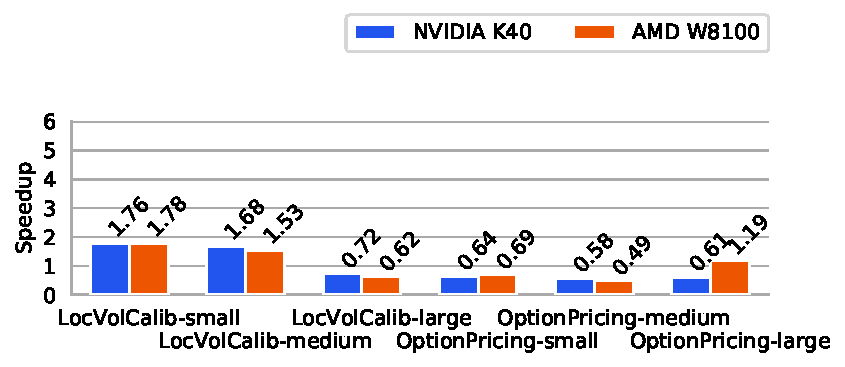
\includegraphics[scale=0.8]{img/finpar.pdf}
  \end{center}


    \begin{itemize}
    \item OpenCL implementations of high quality (written by my
      advisor, so of course).
    \item Datasets have interesting properties.
    \end{itemize}
\end{frame}

\begin{frame}[fragile]
  \frametitle{FinPar: LocVolCalib \\ 1.76$\times$, 1.68$\times$, 0.72$\times$ speedup}

  Core part contains an expression roughly like

\begin{lstlisting}
map (\xs ->
       let xs' = scan (+) 0 xs
       let xs'' = reduce (+) 0 xs'
       let xs''' = map (f xs'') xs'
       in xs)
    xss
\end{lstlisting}

  \begin{itemize}
  \item Should the inner parallism be exploited?  Depends on size of
    \lstinline{xss}.
  \item Smaller two datasets do not have enough \textit{parallelism}
    in the outer \lstinline{map} to saturate the GPU.
  \item Both Futhark and reference implementations focused on the
    largest dataset.
  \end{itemize}

\textbf{Future solution: multi-versioned code.}
\end{frame}

\begin{frame}
  \frametitle{Accelerate}

  \begin{center}
    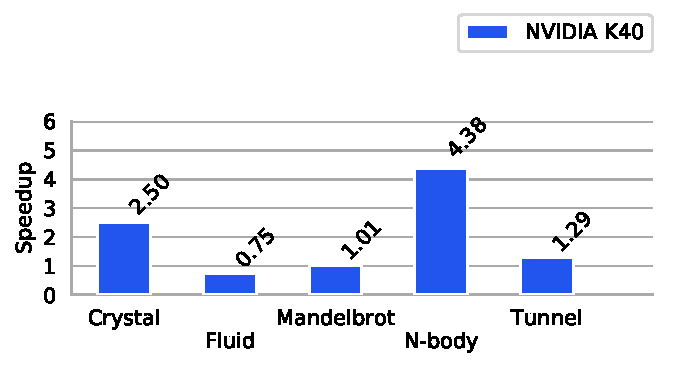
\includegraphics[scale=0.8]{img/accelerate.pdf}
  \end{center}

  \begin{itemize}
  \item High-level parallel array language embedded in Haskell.
  \item Only supports NVIDIA GPUs.
  \item Benchmarks generally pretty simple, with no nested
    parallelism, as it is not supported by Accelerate.
  \end{itemize}

\end{frame}

\begin{frame}[fragile]
  \frametitle{Accelerate: N-body \\ 4.38$\times$ speedup}

\begin{lstlisting}
map (\body -> reduce sum_accel 0 zero_accel
              (map (acceleration body) bodies))
    bodies
\end{lstlisting}

  \begin{itemize}
  \item Inner \lstinline{map-reduce} is sequentialised.
  \item Each thread is looping over the same array: \lstinline{bodies}. \pause
  \item This can be tiled in local memory!
  \item This gives the speedup over accelerate.
  \end{itemize}

\begin{lstlisting}
map (\body ->
      stream_seq (\bodies' ->
                    reduce sum_accel 0 zero_accel
                    (map (acceleration body) bodies'))
                 bodies)
    bodies
\end{lstlisting}

\end{frame}

\begin{frame}
  \frametitle{So it's fast, but is it usable?}

  We can give indirect proof of usability by implementing real(-ish)
  software in Futhark.

\end{frame}

\begin{frame}
  \frametitle{The Enabling Division}

  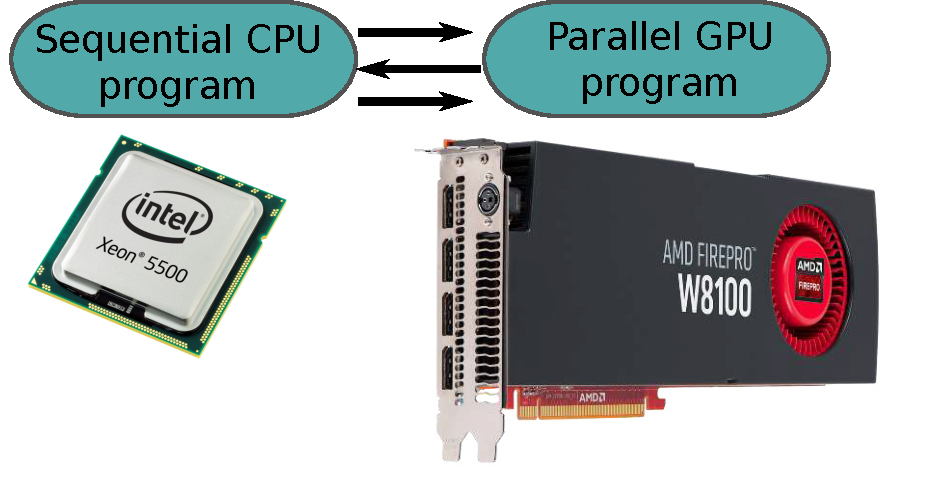
\includegraphics[width=\textwidth]{img/cpu_gpu_division.pdf}

  \bigskip

  The controlling CPU program does \textit{not} have to be fast.  It
  can be generated in a language that is \textit{convenient}.

\end{frame}

\begin{frame}[fragile]
  \frametitle{Compiling Futhark to Python+PyOpenCL}

{\scriptsize
\begin{verbatim}
entry sum_nats (n: i32): i32 =
  reduce (+) 0 [1...n]
\end{verbatim}
}

{\scriptsize
\begin{verbatim}
$ futhark-pyopencl --library sum.fut
\end{verbatim}
}

This creates a Python module \texttt{sum.py} which we can use as follows:

\begin{minipage}{0.49\linewidth}
\begin{lstlisting}[language=none]
$ python
>>> from sum import sum
>>> c = sum()
>>> c.sum_nats(10)
55
>>> c.sum_nats(1000000)
1784293664
\end{lstlisting}

  Good choice for all your integer summation needs!
\end{minipage}\pause
\begin{minipage}{0.49\linewidth}

\includegraphics[width=\linewidth]{img/sanic.jpg}
\end{minipage}

\textit{Or}, we could have our Futhark program return an array
containing pixel colour values, and use Pygame to blit it to the
screen...

\end{frame}

\begin{frame}
  \begin{center}
    \huge CONCLUSIONS
  \end{center}

\vfill

\begin{quote}
  Well, that wasn't so hard! \\\hfill ---Sonic the Hedgehog (Sonic Adventure, 1998)
\end{quote}
\end{frame}

\usebackgroundtemplate{
\tikz[overlay,remember picture] \node[opacity=0.4, at=(current page.center)] {
   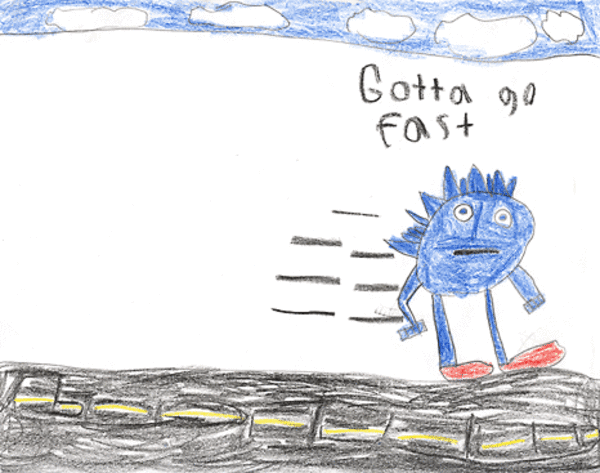
\includegraphics[height=\paperheight,width=\paperwidth]{img/gottagofast.png}};
}

\begin{frame}
  \frametitle{Conclusions}

  \begin{itemize}
  \item The future is parallel, and we need programming models that
    allow us to program with a parallel vocabulary.

  \item Chunking data-parallel operators permit a balance between
    efficient sequential code with in-place updates and all necessary
    parallelism.

  \item Regular nested parallelism can be flattened via loop fission;
    exploiting parallelism while still permitting low-level memory
    access optimisations.

  \item Performance is decent.

  \item The language seems useful.
  \end{itemize}

\end{frame}

\usebackgroundtemplate{}

\begin{frame}
  \begin{center}
    \huge{APPENDICES}
  \end{center}

  \vfill

  \begin{quote}
    Keep it up. There are still lots more left! \\\hfill ---
    Dr. Eggman (Shadow the Hedgehog, 2001)
  \end{quote}
\end{frame}

\begin{frame}
  \frametitle{Validity of Chunking}

  Any fold with an associative operator $\odot$ can be rewritten as:

  \[
   \texttt{fold}\ \odot\ xs\ =\ \texttt{fold}\ \odot\ (\texttt{map}\ (\texttt{fold}\ \odot)\ (\texttt{chunk}\ xs))
 \]

 The trick is to provide a language construct where the user can
 provide a specialised implementation of the \textit{inner} fold,
 which need not be parallel.
\end{frame}

\begin{frame}[fragile]
  \frametitle{Optimising Locality of Reference}

\begin{lstlisting}
map (\x ->
       let zs = map (+x) ys
       in reduce (+) 0 zs)
    xs
\end{lstlisting}

  Only the outer \lstinline{map} is parallel, and all threads are
  reading the same elements of \lstinline{ys}, which can thus be
  cooperatively stored in GPU local memory by collective copying:

\begin{lstlisting}
map (\x ->
       let ys' = local ys
       let zs = map (+x) ys'
       in reduce (+) 0 zs)
    xs
\end{lstlisting}

\end{frame}

\begin{frame}
  \frametitle{Why GPUs?}

  \begin{description}
  \item[\textbf{Cheap}] Easing their programming has a democratising effect, as
    it makes high-performance computation more accessible.
  \item[\textbf{Widespread}] This room contains dozens of GPUs, but likely not
    even a single \textit{programmable} FPGA (unless you brought one).
  \item[\textbf{Restricted}] If Futhark can be translated to GPU
    code, then it can likely also be translated to other platforms.
  \item[\textbf{``Easy''}] The performance guidelines for GPUs are
    fairly straightforward.  Applying them manually is extremely
    tedious and error-prone, but they are a good fit for a compiler.
  \end{description}
\end{frame}

\begin{frame}
  \frametitle{Future Directions}

  \begin{description}
  \item[\textbf{Dataset-sensitive compilation}]\hfill\\
    There is no \textit{one size fits all} for parallelisation.  The
    compiler should generate multiple program versions, and pick the
    optimal one at runtime based on the concrete dataset.
  \item[\textbf{Flexibility}]\hfill\\ Support for irregular problems, such as graph
    algorithms.  Not \textit{at all costs}---other more expressive
    languages already exist.  Futhark's gotta go fast.
  \item[\textbf{Clusters}]\hfill\\ Single computers are so 2000---transparent
    distributed computing on moderately sized clusters would be
    useful.
  \item[\textbf{Heterogeneity}]\hfill\\ Splitting computation between
    both CPU and GPU.
  \end{description}
\end{frame}

\begin{frame}[fragile]
  \frametitle{Futhark?}

  % \Draw(x,y,length,angle) Angle must be -90 .. 90
\def\Draw(#1,#2,#3,#4){{
\put(#1,#2){\rotatebox{#4}{\rule[-0.5pt]{#3\unitlength}{1pt}}}
}}

\begin{center}

\setlength{\unitlength}{1.9em}
\huge
\begin{picture}(33,5)(0,0.1)
\put(1,0.8){f}

\Draw(1,2,2,90)
\Draw(1,3,1.41,45)
\Draw(1,3.5,0.71,45)

\put(3,0.8){u}

\Draw(3,2,2,90)
\Draw(3,4,1,-45)
\Draw(3.7,2,1.3,90)

\put(4.8,0.8){th}

\Draw(5,2,2,90)
\Draw(5,2.5,0.71,45)
\Draw(5,3.5,0.71,-45)

\put(7,0.8){a}

\Draw(7,2,2,90)
\Draw(7,3,0.71,-45)
\Draw(7,3.5,0.71,-45)

\put(9,0.8){r}

\Draw(9,2,2,90)
\Draw(9,4,0.85,-45)
\Draw(9,2.8,0.85,45)
\Draw(9,2.8,1.13,-45)


\put(11,0.8){k}

\Draw(11,2,2,90)
\Draw(11,3.3,1,45)
\end{picture}
\end{center}

\bigskip
(With thanks to Torben Mogensen.)

\end{frame}

\end{document}

%%% Local Variables:
%%% mode: latex
%%% TeX-master: t
%%% End:
